% =====================================================================
% main.tex - Entrega 2 PLN: EDA avanzado, representacion de textos y
% propuesta metodologica. Corpus de sentencias de la Corte Constitucional
% de Colombia (1992-2021).
% Clase tg_usta (NO modificar tg_usta.cls). Compilar con pdflatex+bibtex
% (ver README_compilar.md). Version F4b: marcadores TODO(F4b) resueltos
% con las cifras del notebook ejecutado.
% =====================================================================
\documentclass[11pt]{tg_usta}

\usepackage[utf8]{inputenc}
\usepackage[T1]{fontenc}
\usepackage{anysize}
\usepackage{graphicx}
\usepackage{subcaption}
\usepackage{booktabs}
\usepackage{url}

\marginsize{1in}{1in}{1in}{1in} %% Margenes de 1 pulgada (NO MODIFICAR)

% ---------------------------------------------------------------------
% Informe con muchas figuras y tablas: se permite hasta 3 flotantes
% arriba y 4 en total por pagina para reducir paginas de solo flotantes
% (ajuste de maquetacion; no altera margenes ni contenido).
% ---------------------------------------------------------------------
\setcounter{topnumber}{3}
\setcounter{totalnumber}{4}
\renewcommand{\topfraction}{0.85}
\renewcommand{\textfraction}{0.10}

% ---------------------------------------------------------------------
% Figuras: la entrega mantiene las figuras en entrega_2_eda/figuras/.
% Se busca primero alli y luego junto al informe.
% ---------------------------------------------------------------------
\graphicspath{{../figuras/}{./figuras/}}

% ---------------------------------------------------------------------
% Nota sobre las citas: tg_usta.cls carga el paquete `harvard', que
% redefine \cite y solo resuelve referencias de estilos propios
% (agsm/dcu). Para poder usar el estilo apalike (pedido en la guia de la
% entrega) se restaura aqui el \cite estandar del kernel de LaTeX, que
% resuelve las etiquetas \bibcite generadas por apalike.bst (formato
% [Autor, anio]). No se modifican las citas de harvard: simplemente se
% sustituye \cite por la definicion original del kernel.
\makeatletter
\renewcommand{\cite}{\@ifnextchar[{\@tempswatrue\@citex}{\@tempswafalse\@citex[]}}
\makeatother

\begin{document}

% =====================================================================
% PORTADA / ENCABEZADO
% =====================================================================
\title[maintitle = Análisis de sentencias de la Corte Constitucional de Colombia (1992--2021),
       secondtitle = {Entrega 2: EDA avanzado, representación de textos y propuesta metodológica}]

\begin{authors}[Rivera, Carrillo, Garnica \& Prieto]

% Pontificia Universidad Javeriana, Bogotá (Colombia)
\author[firstname = Erika Valeria,
        surname = Rivera Jimenez,
        email = riveraev@javeriana.edu.co]

\author[firstname = Julian Guillermo,
        surname = Carrillo Meneses,
        email = carrillojuliang@javeriana.edu.co]

\author[firstname = Carlos Andres,
        surname = Garnica Salazar,
        email = carlos\_garnicas@javeriana.edu.co]

\author[firstname = Oscar Andres,
        surname = Prieto Moreno,
        email = o-prieto@javeriana.edu.co]

\end{authors}

\begin{center}\footnotesize Pontificia Universidad Javeriana, Bogotá, Colombia\end{center}

\begin{mainabstract}

Esta segunda entrega profundiza el análisis del corpus de 23.742 sentencias de la Corte Constitucional de Colombia (1992--2021), entrega el corpus en su versión medida y define la representación de los textos y la metodología de modelado del proyecto. Primero se documentan las modificaciones respecto a la Entrega 1: el corpus se persiste como conjunto de datos medido (\emph{parquet} con texto, texto limpio y métricas por documento), se incorpora un EDA avanzado ---n-gramas y colocaciones con validación manual, lemas, \emph{stems} y categorías gramaticales, diversidad léxica MTLD, evolución por periodos, granularidad y evaluación de recursos léxicos--- y se valida con evidencia la unidad de análisis (sentencia completa). Segundo, se comparan las familias de representación (bolsa de palabras, TF-IDF, \emph{embeddings} y representaciones contextuales) y se selecciona y calcula TF-IDF sobre lemas como representación principal (matriz de 23.742 $\times$ 100.000 rasgos). Tercero, se propone una metodología de clasificación supervisada multi-clase con particiones estratificadas, criterios anti-\emph{leakage} y comparación entre modelos lineales y \emph{transformers} en español. Los resultados caracterizan el carácter formulaico del género, una diversidad léxica decreciente entre 1992 y 2021, un recambio temático visible en el vocabulario de la última década y la viabilidad de la sentencia completa como unidad de análisis.\\\\
\textit{\textbf{Palabras clave:}} procesamiento de lenguaje natural, lenguaje jurídico, Corte Constitucional de Colombia, EDA avanzado, diversidad léxica, representación de textos, TF-IDF, clasificación de documentos legales.

\end{mainabstract}

% =====================================================================
% SECCION 1: INTRODUCCION
% =====================================================================
\section{Introducción}

\subsection{Contexto y motivación}
Este proyecto aborda el análisis computacional de las sentencias de la Corte Constitucional de Colombia emitidas entre 1992 y 2021 mediante técnicas de procesamiento de lenguaje natural (PLN). El corpus de trabajo reúne 23.742 providencias de tres tipos ---tutela (T, 17.099), constitucionalidad (C, 6.246) y unificación (SU, 397)---, obtenidas del repositorio público de Hugging Face \emph{Manuel/sentencias-corte-cons-colombia-1992-2021} \cite{manuel2022sentencias}. Se trata de un corpus de ``pocos documentos pero muy extensos'': cada sentencia promedia $\approx$ 11.000 palabras, con estructura discursiva formal, terminología especializada, fórmulas de estilo estables y abundantes citas normativas y jurisprudenciales; la literatura sobre sentencias largas advierte que este perfil exige cautela al interpretar los conteos globales y recomienda complementarlos con estadísticas por documento \cite{soh2019legalarea}.

La Entrega 1 consolidó ese corpus: documentó su depuración, ejecutó una textometría básica sobre la totalidad de los documentos y dejó planteadas las líneas de trabajo posteriores (lematización, representaciones vectoriales y clasificación automática). Esta segunda entrega responde al propósito del enunciado de la Entrega 2: profundizar en el análisis del corpus, mostrar la representación de los textos según el contexto del proyecto y proponer una metodología de modelado inicial. La motivación es doble. Por un lado, la caracterización léxica y morfológica es un insumo directo para decidir cómo representar los documentos y qué rasgos conservar; por otro, los recursos legales anotados en español para América Latina son escasos \cite{loffler2025predicting}, de modo que un corpus colombiano depurado, medido y documentado constituye un aporte en sí mismo.

\subsection{Objetivo del proyecto}
El objetivo general del proyecto es construir un sistema de apoyo que, dada una sentencia de la Corte Constitucional de Colombia: (i) valide que se trata de una providencia; (ii) determine su área temática constitucional; (iii) identifique los artículos de la Constitución Política (CP) en los que se sustenta; y (iv) la sitúe en su contexto jurisprudencial. El sistema se concibe como una herramienta de apoyo a la consulta y al análisis especializado, no como un sustituto de la interpretación jurídica.

Esta entrega no ejecuta los modelos de la fase final: prepara el terreno para ellos. Concretamente, entrega el conjunto de datos medido (requisito 3 del enunciado), el análisis exploratorio avanzado (requisito 2), la representación de los textos (requisito 4) y la propuesta metodológica (requisito 5), además de las correcciones y modificaciones respecto a la Entrega 1 (requisito 1) y del formato de entrega con informe y carpeta de datos (requisito 7). El alcance temporal se mantiene estrictamente en 1992--2021; el año 2021 es parcial (20 documentos).

\subsection{Aportes de esta entrega y organización del documento}
Los aportes se organizan así. La sección \ref{sec:cambios} documenta las correcciones y modificaciones respecto a la Entrega 1, verificadas contra el informe y los artefactos de esa entrega, y explica las razones de cada cambio. La sección \ref{sec:corpus} describe la fuente, la depuración, el \emph{pipeline} de limpieza y el conjunto de datos medido que se adjunta, junto con las medidas globales. La sección \ref{sec:eda} presenta el EDA avanzado: n-gramas y colocaciones con validación manual, diversidad léxica (MTLD), morfología (lemas, \emph{stems} y categorías gramaticales), evolución léxica por periodos, evaluación de recursos léxicos y granularidad. La sección \ref{sec:representacion} compara las familias de representación y justifica la decisión por TF-IDF sobre lemas. La sección \ref{sec:metodologia} formula la propuesta metodológica de modelado. La sección \ref{sec:conclusiones} cierra con las conclusiones.

% =====================================================================
% SECCION 2: CORRECCIONES Y MODIFICACIONES
% =====================================================================
\section{Correcciones y modificaciones respecto a la Entrega 1}
\label{sec:cambios}

Esta sección responde al requisito 1 del enunciado: indicar qué ajustes se realizaron al corpus, a las visualizaciones o al planteamiento inicial, y explicar brevemente las razones. Cada cambio candidato se verificó contra el informe de la Entrega 1 y sus artefactos (notebook ejecutado, \texttt{metricas.json}, \texttt{eda\_extendido/}); se reportan únicamente cambios reales. Las cifras canónicas de la Entrega 1 no requirieron corrección: el EDA extendido reproduce el tamaño del corpus (23.742 documentos) y la distribución por tipos (T 17.099, C 6.246, SU 397), y las medidas globales de palabras crudas y limpias se mantienen (sección \ref{sec:medidas}). Los seis cambios efectivos se agrupan en tres frentes: el conjunto de datos entregado, la profundidad del análisis y las decisiones de planteamiento.

\subsection{Del anexo de muestra al conjunto de datos medido}
La Entrega 1 adjuntó una muestra estratificada de 25 sentencias (17 T, 6 C y 2 SU) con fines de revisión, y conservó los conteos por documento en un archivo de metadatos sin texto (\texttt{df\_metadatos.csv}: identificador, tipo, número, año y conteos de palabras). En esta entrega el corpus completo se persiste como \texttt{datos/corpus\_medido.parquet}: 23.742 filas con el texto original, el texto limpio y las métricas por documento (sección \ref{sec:dataset}). La razón es doble: el enunciado exige entregar el corpus en su versión actualizada, preprocesado y acompañado de sus métricas, en un formato legible que incluya las variables relevantes; además, el \emph{parquet} se convierte en el insumo único y trazable del análisis de representación y de la fase de modelado, lo que reduce el riesgo de inconsistencias entre etapas.

\subsection{EDA avanzado y nuevas visualizaciones}
La Entrega 1 reportó textometría básica (medidas globales, top-20 con y sin palabras vacías, distribución temporal y nubes de palabras). Sobre el mismo corpus se calculó un EDA extendido ---n-gramas, colocaciones, lemas y \emph{stems}, categorías gramaticales (POS), diversidad léxica MTLD, granularidad y evaluación de recursos léxicos--- cuyos artefactos quedaron disponibles en \texttt{resultados/eda\_extendido/}, pero que no alcanzó a reportarse en el informe anterior. Esta entrega lo incorpora con su lectura analítica completa (sección \ref{sec:eda}), tal como pide el requisito 2 del enunciado. En consecuencia, se añaden siete visualizaciones nuevas (n-gramas bi/trigramas, colocaciones por razón de verosimilitud, lemas frente a \emph{stems}, distribución POS, distribución de MTLD, granularidad y nube global de contenido) y se conservan las figuras de la Entrega 1, cuyas cifras siguen vigentes.

\subsection{Unidad de análisis validada con evidencia}
La Entrega 1 analizaba implícitamente la sentencia completa como unidad, sin justificarlo. Antes de fijar la representación y la metodología, esta entrega evaluó tres granularidades posibles (sentencia, párrafo y subsentencia) con un criterio pre-registrado: la subsentencia solo se propondría como unidad si superaba en al menos 15 puntos porcentuales la pureza temática de la sentencia completa (sección \ref{sec:granularidad}). El resultado (4,64\,\% de subsentencias con marcador frente a 97,17\,\% de sentencias) no superó el criterio, de modo que se mantiene la sentencia completa como unidad de análisis, ahora con evidencia y no por omisión. La razón del experimento es evitar que una decisión costosa de revertir ---segmentar 23.742 documentos para modelar fragmentos--- se tomara sin medir su efecto sobre la señal temática disponible.

\subsection{Cumplimiento del análisis por periodos prometido en la Entrega 1}
La Entrega 1 anunció que ``el análisis cuantitativo de la evolución léxica por periodos se abordará en la entrega 2''. Esta entrega cumple esa promesa con un contraste de tres periodos (1992--2001, 2002--2011 y 2012--2021) mediante razones de \emph{log-odds} binarias con suavizado add-0,5 \cite{hamilton2016diachronic}, acompañado de la evidencia cualitativa de las nubes anuales y de la serie de diversidad léxica (secciones \ref{sec:periodos} y \ref{sec:mtld}). El análisis diacrónico del discurso judicial está respaldado por la literatura como una vía para detectar cambios de agenda y de estilo de redacción en los tribunales \cite{raj2026collective}.

\subsection{Representación definida y propuesta metodológica}
La Entrega 1 dejó como trabajo futuro ``representaciones del texto (TF-IDF y vectores densos)'' y ``experimentos de clasificación automática por tipo y temática''. Esta entrega define y justifica la representación principal (TF-IDF sobre lemas, sección \ref{sec:decision}) y formula la propuesta metodológica de los modelos (sección \ref{sec:metodologia}): tipo de tarea, etiquetas, particiones, criterios anti-\emph{leakage}, modelos a comparar y criterios de evaluación. Se trata de un cambio de estado del proyecto ---de la exploración descriptiva al diseño experimental--- y no de una rectificación de la Entrega 1, cuyos resultados siguen siendo la línea base del proyecto.

% =====================================================================
% SECCION 3: CORPUS Y PREPROCESAMIENTO
% =====================================================================
\section{Corpus y preprocesamiento}
\label{sec:corpus}

\subsection{Fuente y depuración}
El corpus proviene del repositorio abierto \emph{sentencias-corte-cons-colombia-1992-2021}, publicado por el usuario \emph{Manuel} en el Hugging Face Hub bajo licencia CC-BY-4.0 \cite{manuel2022sentencias}. El archivo original es un CSV plano de 1,68\,GB en UTF-8 (\texttt{Juris1992\_2022.csv}) con dos columnas, un identificador y el texto completo de la providencia; su nombre sugiere cobertura hasta 2022, pero la cobertura real es 1992--2021: no hay documentos de 2022 y el año 2021 es parcial, con solo 20 sentencias. La fuente primaria de los textos es la relatoría de la Corte Constitucional de Colombia.

La depuración siguió el procedimiento documentado en la Entrega 1. El CSV contiene 23.750 filas; el identificador de la sentencia (por ejemplo, \texttt{T-293/97}) y el año de emisión se extraen del encabezado mediante expresiones regulares sobre el patrón \emph{Sentencia T-293/97}, con una tasa de éxito del 99,97\,\% (23.742 de 23.750). Las 8 filas restantes se excluyeron y documentaron: 6 corresponden a autos (no sentencias) y 2 a fragmentos HTML residuales del proceso de recolección. El corpus de análisis queda así conformado por 23.742 sentencias. El universo documental subyacente ya había sido explorado computacionalmente: Anzola Cortés analizó más de 6.000 sentencias de constitucionalidad (1992--2020) con minería de datos y documentó los problemas estructurales de estos textos (fórmulas de estilo y referencias embebidas) \cite{anzolaCortes2021algoritmos}. La tabla \ref{tab:ficha} resume la ficha del corpus.

\begin{table}[htbp]
    \centering
    \caption{Ficha del corpus de análisis (1992--2021).}
    \label{tab:ficha}
    \begin{tabular}{p{0.30\textwidth}p{0.62\textwidth}}
        \toprule
        \textbf{Elemento} & \textbf{Valor} \\
        \midrule
        Origen & Hugging Face: \emph{Manuel/sentencias-corte-cons-colombia-1992-2021} (CC-BY-4.0) \cite{manuel2022sentencias} \\
        Archivo fuente & \texttt{Juris1992\_2022.csv} (1,68\,GB; 23.750 filas; columnas ID y Texto) \\
        Corpus de análisis & 23.742 sentencias \\
        Tipos de providencia & T: 17.099 (72,02\,\%); C: 6.246 (26,31\,\%); SU: 397 (1,67\,\%) \\
        Cobertura temporal & 1992--2021 (2021 parcial: 20 documentos) \\
        Exclusiones & 8 filas (6 autos; 2 fragmentos HTML) \\
        Persistencia & \texttt{datos/corpus\_medido.parquet} (texto, texto limpio y métricas por documento) \\
        \bottomrule
    \end{tabular}
\end{table}

\subsection{Pipeline de limpieza reproducible}
El \emph{pipeline} de limpieza se aplicó por etapas medibles y se documenta como decisión metodológica, pues la literatura muestra que el preprocesamiento altera los resultados y que su efecto depende del corpus y de la tarea \cite{hacohenKerner2020influence}. La tabla \ref{tab:pipeline} lista los ocho pasos, idénticos a los de la Entrega 1 para garantizar la comparabilidad de las cifras. Dos decisiones merecen énfasis. Primero, la normalización Unicode (NFD con retiro de diacríticos) protege la letra \emph{ñ} antes de descomponer, de modo que las grafías del corpus quedan sin tildes pero conservan la virgulilla (\emph{artículo} $\rightarrow$ \emph{articulo}; \emph{año} $\rightarrow$ \emph{año}). Segundo, la lista de palabras vacías del español de NLTK se sometió a la misma transformación que el corpus: quedan 306 formas efectivas sin tildes, pues 84 formas acentuadas del conjunto original (\emph{más}, \emph{está}, \emph{cómo}, \ldots) se normalizaron igual que el texto; de otro modo, esas formas dejarían de filtrarse y contaminarían los conteos.

\begin{table}[htbp]
    \centering
    \caption{Pasos del \emph{pipeline} de limpieza aplicado a cada documento.}
    \label{tab:pipeline}
    \small
    \begin{tabular}{clp{0.46\textwidth}}
        \toprule
        \textbf{\#} & \textbf{Paso} & \textbf{Efecto} \\
        \midrule
        1 & Minúsculas & \emph{Sentencia} y \emph{SENTENCIA} $\rightarrow$ \emph{sentencia} \\
        2 & Protección de la \emph{ñ} & centinela temporal antes de la descomposición NFD \\
        3 & Normalización NFD y retiro de diacríticos & \emph{artículo} $\rightarrow$ \emph{articulo} \\
        4 & Filtro de caracteres \texttt{[a-zñ]} & elimina dígitos, puntuación y símbolos \\
        5 & Colapso de espacios & series de espacios $\rightarrow$ un espacio \\
        6 & Tokenización por separación en espacios & token exacto = palabra alfabética \\
        7 & Filtro de ruido & descarta \emph{t}, \emph{c}, \emph{p} (restos de claves y citas de página) y la abreviatura \emph{art} \\
        8 & Palabras vacías normalizadas & 306 formas, con la misma normalización del corpus \\
        \bottomrule
    \end{tabular}
\end{table}

El paso 7 ---denominado \emph{filtro de ruido}--- evita que tokens de un solo carácter generados por la limpieza (la clave \texttt{T-001/21} deja el token \emph{t}; \texttt{C-123/19}, el token \emph{c}; las citas de página \texttt{p.~45}, el token \emph{p}) escalen en los conteos de frecuencia, y elimina la abreviatura de cita \emph{art}. Adicionalmente, para las visualizaciones de nubes se retiraron 65 formas de vocabulario jurídico-procesal propio del género (\emph{sentencia(s)}, \emph{corte}, \emph{constitucional}, \emph{derecho(s)}, \emph{tutela(s)}, \emph{articulo(s)}, \emph{ley(es)}, \emph{magistrado(s)}, \emph{ponente}, \emph{expediente(s)}, entre otras); la literatura sobre corpus judiciales en español justifica complementar las palabras vacías gramaticales con este vocabulario de género cuando se quiere observar el contenido temático \cite{barbosaBecerra2021comportamiento,gonzalezGonzalez2023automatic}.

\subsection{Conjunto de datos medido}
\label{sec:dataset}
El conjunto de datos medido es el entregable principal del requisito 3 del enunciado. Se adjunta a este informe en la carpeta \texttt{datos/} con el nombre \texttt{corpus\_medido.parquet}, un archivo columnar legible que reúne las 23.742 sentencias con su texto original, su texto limpio y las métricas calculadas por documento. La tabla \ref{tab:diccionario} presenta el diccionario de datos del esquema. El conjunto se acompaña de una muestra estratificada en CSV (\texttt{corpus\_medido\_muestra.csv}: 100 filas por tipo y década con semilla 42, que añade las columnas \texttt{decada} y \texttt{texto\_limpio\_preview}) para inspección rápida, y del diccionario de datos en formato Markdown (\texttt{diccionario\_datos.md}, 14 variables: las 12 del \emph{parquet} más las 2 de la muestra); además, la carpeta incluye una copia de los contadores de lemas por documento (\texttt{lemas\_por\_doc.parquet}) para reproducibilidad del análisis morfológico.

\begin{table}[htbp]
    \centering
    \caption{Diccionario de datos de \texttt{corpus\_medido.parquet} (23.742 filas).}
    \label{tab:diccionario}
    \begin{tabular}{llp{0.55\textwidth}}
        \toprule
        \textbf{Columna} & \textbf{Tipo} & \textbf{Descripción} \\
        \midrule
        \texttt{id} & cadena & identificador del documento en el corpus (clave estable del \emph{join}) \\
        \texttt{tipo} & cadena & tipo de providencia: T (tutela), C (constitucionalidad), SU (unificación) \\
        \texttt{numero} & entero & número de la sentencia (p.~ej., 001) \\
        \texttt{ano} & entero & año de emisión (1992--2021) \\
        \texttt{texto} & cadena & texto crudo completo de la sentencia (promedio $\approx$ 11.000 palabras) \\
        \texttt{texto\_limpio} & cadena & texto normalizado (minúsculas, sin diacríticos, solo letras y espacios; tokens de ruido filtrados) \\
        \texttt{n\_chars\_texto} & entero & caracteres del texto crudo \\
        \texttt{n\_palabras\_raw} & entero & palabras por separación de espacios del texto crudo (incluye números y claves) \\
        \texttt{n\_palabras\_clean} & entero & tokens alfabéticos tras la limpieza y el filtro de ruido \\
        \texttt{n\_stopwords} & entero & tokens limpios que son palabras vacías gramaticales (306 formas normalizadas) \\
        \texttt{n\_lemas} & entero & lemas por documento (spaCy \texttt{es\_core\_news\_md}) \\
        \texttt{mtld} & real & diversidad léxica MTLD del documento (umbral 0,72) \\
        \bottomrule
    \end{tabular}
\end{table}

La construcción del archivo se validó con aserciones duras contra las cifras canónicas del corpus: 23.742 filas, 23.742 identificadores únicos y sin valores nulos en las claves (\texttt{id}, \texttt{tipo}, \texttt{numero}, \texttt{ano}) ni en \texttt{n\_lemas}/\texttt{mtld}; las sumas quedan reconciliadas con las medidas globales de la sección \ref{sec:medidas} (palabras crudas 260.988.316, palabras limpias 250.012.101, palabras vacías 121.205.437 y 248.533.344 lemas totales), y el texto crudo suma 1.640.749.780 caracteres. El archivo final ocupa 1.544,7\,MB. La muestra estratificada quedó conformada por 100 documentos (72 T, 24 C y 4 SU) distribuidos por tipo y década, y el diccionario de datos documenta cada variable con su tipo, descripción, ejemplo real y fuente.

\subsection{Medidas globales}
\label{sec:medidas}
La tabla \ref{tab:medidas} resume las medidas textuales del corpus. Todas las cifras corresponden al conteo real sobre las 23.742 sentencias (no a extrapolaciones de muestras). Tras la limpieza, los tokens alfabéticos ascienden a 250.012.101; al remover las palabras funcionales quedan 128.806.664 tokens, de modo que las palabras vacías representan el 48,48\,\% del corpus limpio. El vocabulario de formas del análisis morfológico es de 224.468 tipos, que se reducen a 195.959 lemas (87,3\,\%) y a 121.696 \emph{stems} (54,2\,\%) (sección \ref{sec:morfologia}).

\begin{table}[htbp]
    \centering
    \caption{Medidas globales del corpus de análisis (23.742 sentencias, 1992--2021).}
    \label{tab:medidas}
    \begin{tabular}{lr}
        \toprule
        \textbf{Medida} & \textbf{Valor} \\
        \midrule
        Documentos & 23.742 \\
        Palabras crudas (\emph{raw}) & 260.988.316 \\
        Palabras normalizadas (limpias) & 250.012.101 \\
        Palabras vacías (\emph{stopwords}) & 121.205.437 (48,48\,\% de las limpias) \\
        Palabras sin palabras vacías & 128.806.664 \\
        Promedio de palabras crudas por documento & 10.992,68 \\
        Promedio de palabras limpias por documento & 10.530,37 \\
        Mediana de lemas por documento (EDA) & 7.116 (p25: 3.959; p75: 12.654) \\
        Mediana de palabras limpias por documento (EDA) & 7.158 \\
        Vocabulario de formas (EDA morfológico) & 224.468 tipos \\
        Lemas / \emph{stems} (EDA morfológico) & 195.959 / 121.696 tipos \\
        \bottomrule
    \end{tabular}
\end{table}

La figura \ref{fig:top20} presenta el top-20 de palabras más frecuentes, con y sin palabras vacías. Con palabras vacías, el top-5 lo encabezan \emph{de} (22.543.375), \emph{la} (14.299.738), \emph{el} (8.225.551), \emph{que} (7.505.218) y \emph{en} (7.208.184); la caída brusca de las frecuencias es consistente con la ley de Zipf y con el peso de las palabras funcionales. Sin palabras vacías emerge el léxico jurídico dominante: \emph{articulo} (947.616), \emph{derecho} (898.926), \emph{ley} (809.313), \emph{corte} (760.197), \emph{sentencia} (736.326), \emph{derechos} (718.194), \emph{constitucional} (689.709) y \emph{tutela} (649.302). Las grafías sin tilde son efecto de la normalización descrita en la sección \ref{sec:corpus}. La figura \ref{fig:por_anio} muestra la distribución temporal: el volumen es relativamente estable entre 1999 y 2014, con un rango de 941 (2013) a 992 (2002) providencias anuales, desciende progresivamente entre 2015 y 2020 y colapsa en 2021 (20 documentos), evidencia de la cobertura parcial de ese año. La figura \ref{fig:nube_global} resume el léxico de contenido en una nube global construida tras retirar las palabras vacías gramaticales y las 65 formas de vocabulario de género.

La longitud de los documentos merece una lectura propia, porque condiciona la interpretación de los conteos globales y la comparabilidad entre documentos. La figura \ref{fig:longitudes} presenta ese perfil sobre las palabras limpias. El histograma (izquierda) muestra una distribución de cola larga y asimetría positiva: la mediana es de 7.158 palabras, muy por debajo de la media (10.530,37), y el extremo superior alcanza 451.252 palabras. El diagrama de caja por tipo (derecha) añade una diferencia sistemática: las tutelas son las más cortas (mediana 6.329), las sentencias de constitucionalidad ocupan una posición intermedia (9.830) y las de unificación son las más extensas (21.626), más del triple que las tutelas. El corpus combina, así, una mayoría de documentos de tamaño moderado con una minoría de documentos excepcionalmente largos y con brechas de longitud entre tipos; por eso las comparaciones por tipo y por periodo se apoyan en estadísticas por documento y en medidas relativas, y no solo en las sumas globales.

La composición por tipo de providencia completa el retrato del corpus. La figura \ref{fig:tipos} recapitula los totales ---tutelas 17.099 (72,0\,\%), constitucionalidad 6.246 (26,3\,\%) y unificación 397 (1,7\,\%)--- y añade su evolución anual apilada entre 1992 y 2021: las tutelas dominan todos los años del periodo, mientras que las C y las SU aportan una fracción minoritaria y relativamente estable, y el bloque de 2021 aparece truncado por corresponder a un año parcial (20 documentos). Este desbalance condiciona la lectura de los n-gramas más frecuentes (sección \ref{sec:ngramas}) y es el punto de partida de las particiones estratificadas y de las métricas macro de la propuesta metodológica (sección \ref{sec:metodologia}).

\begin{figure}[htbp]
    \centering
    \begin{subfigure}[t]{0.48\linewidth}
        \centering
        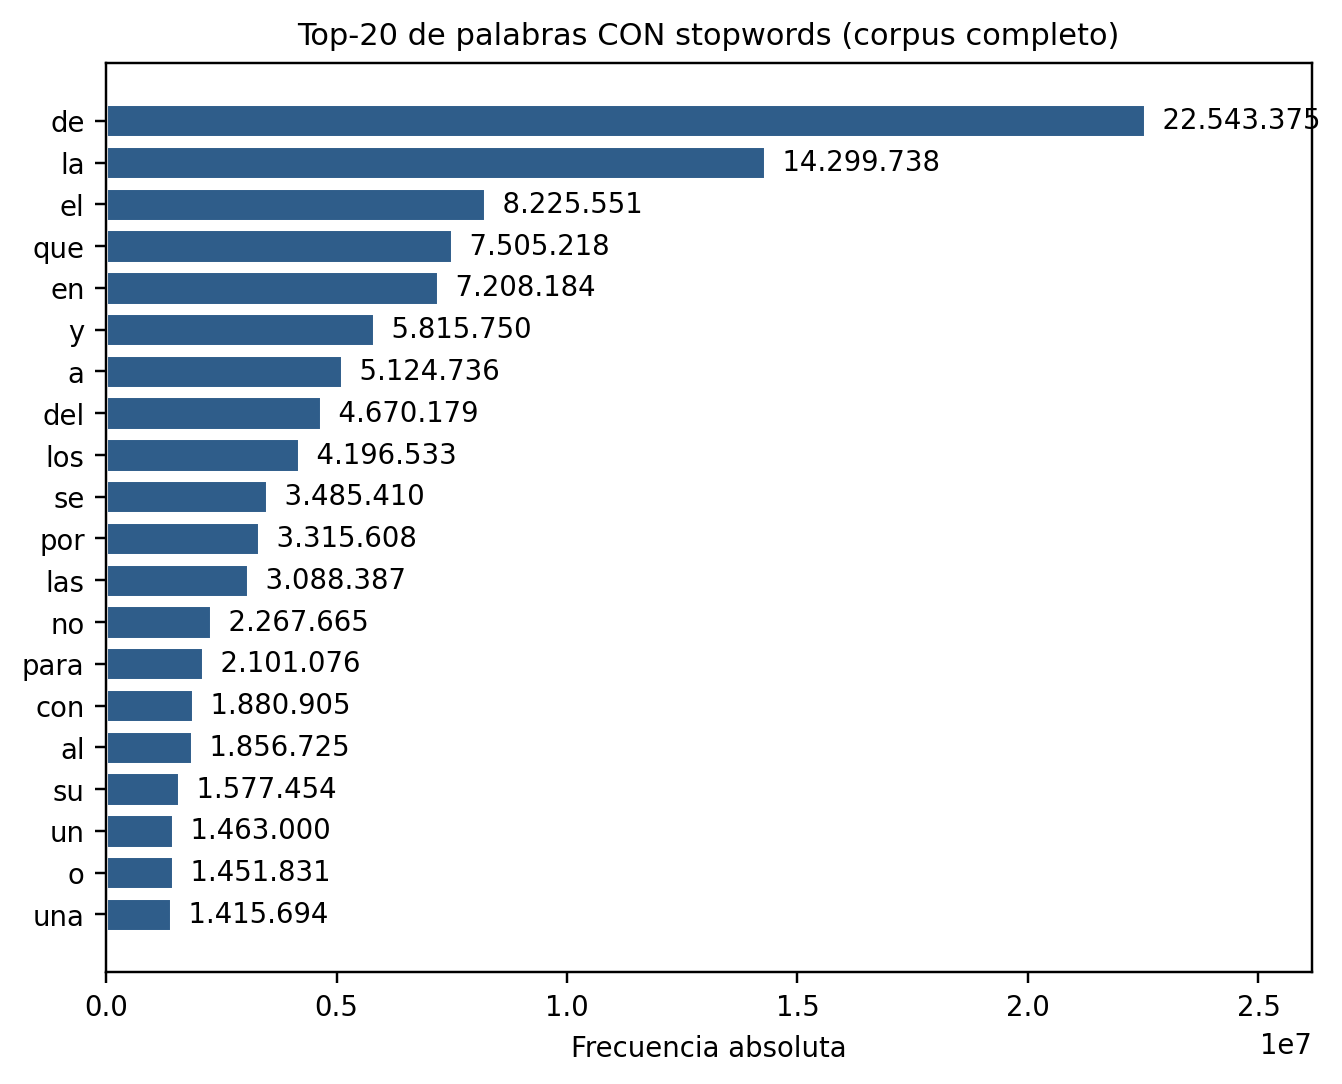
\includegraphics[width=\linewidth]{fig_top20_con_stopwords.png}
        \caption{Con palabras vacías gramaticales.}
        \label{fig:top20_con}
    \end{subfigure}%
    \hfill
    \begin{subfigure}[t]{0.48\linewidth}
        \centering
        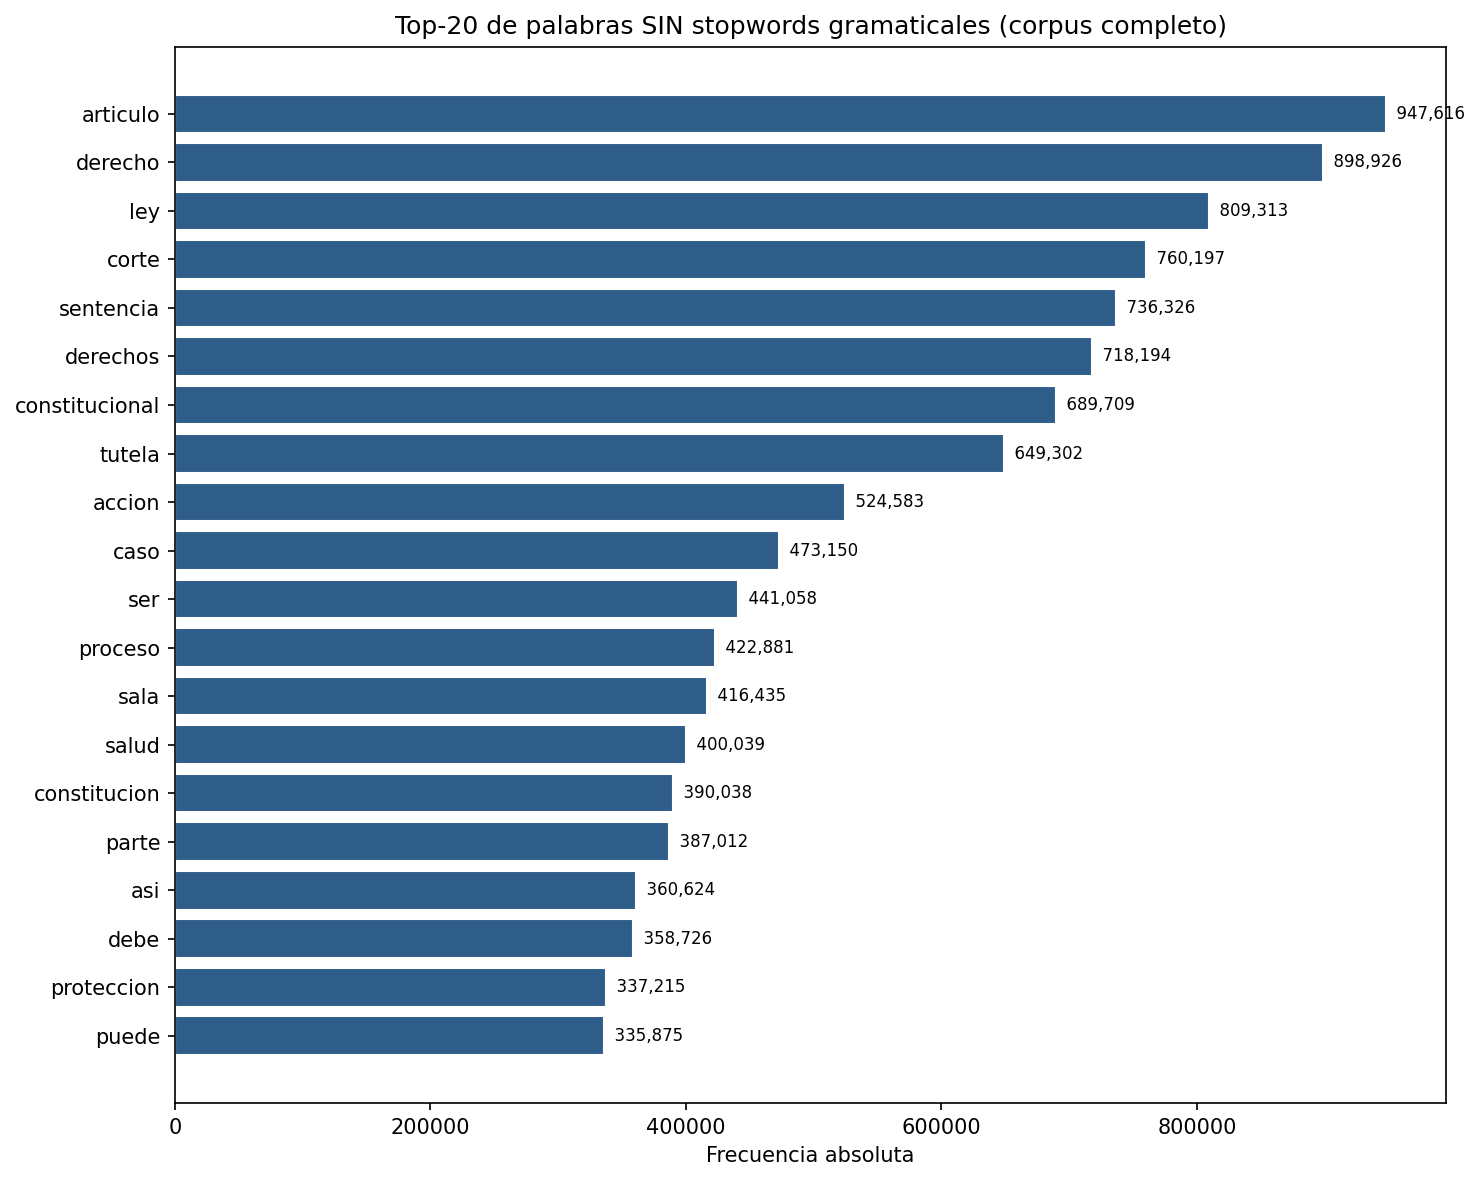
\includegraphics[width=\linewidth]{fig_top20_sin_stopwords.png}
        \caption{Sin palabras vacías gramaticales.}
        \label{fig:top20_sin}
    \end{subfigure}
    \caption{Top-20 de palabras más frecuentes del corpus completo (23.742 sentencias).}
    \label{fig:top20}
\end{figure}

\begin{figure}[htbp]
    \centering
    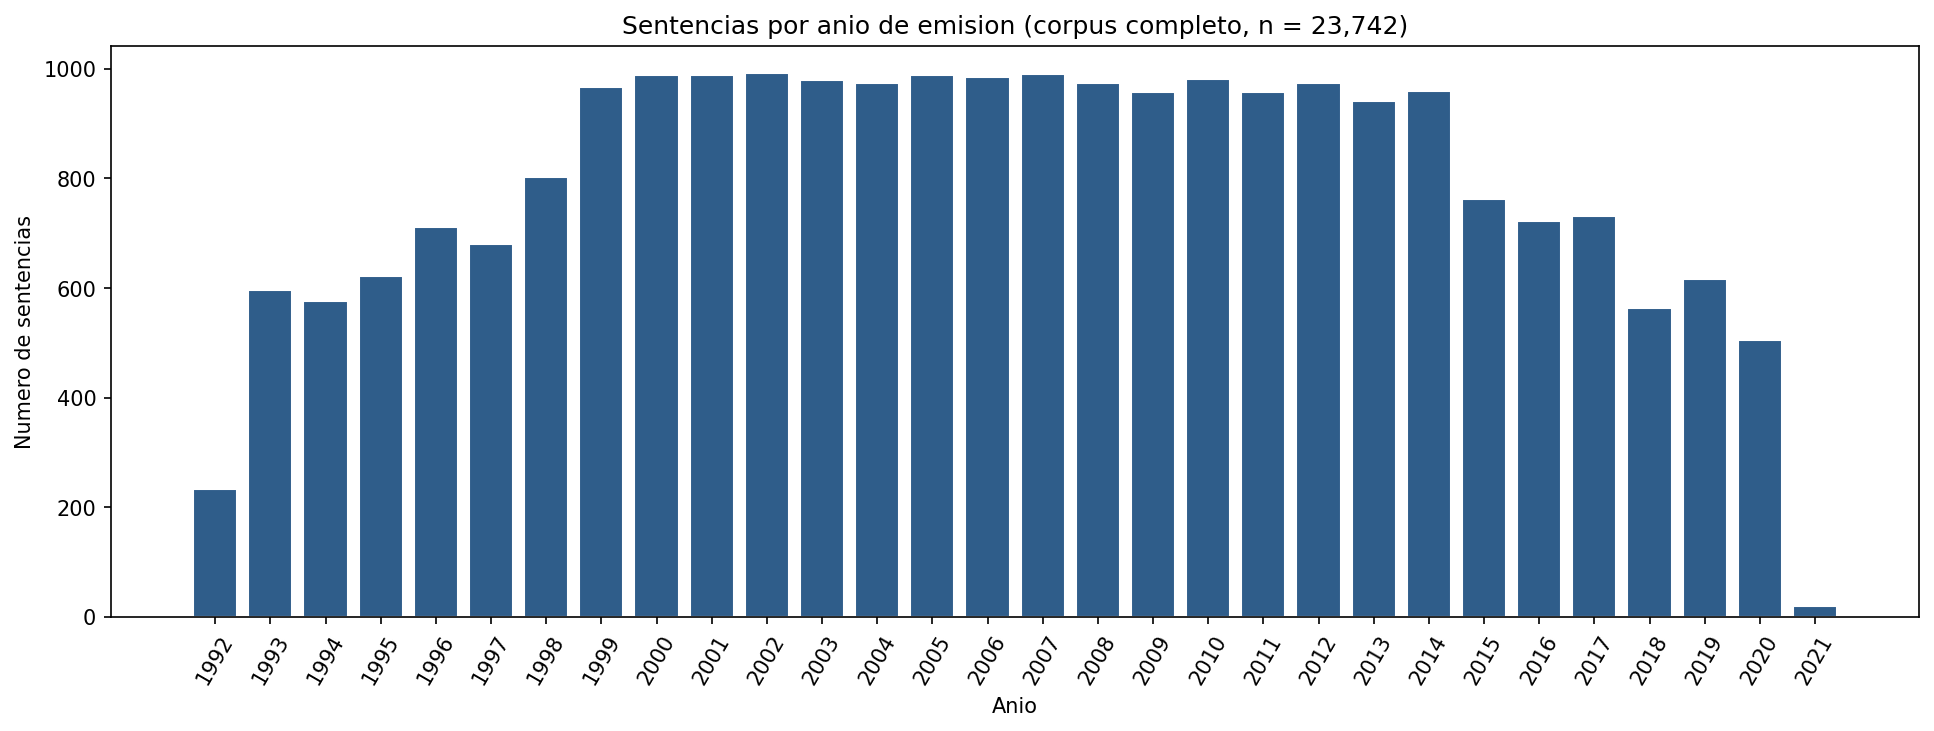
\includegraphics[width=0.75\linewidth]{fig_sentencias_por_anio.png}
    \caption{Sentencias del corpus por año de emisión, 1992--2021.}
    \label{fig:por_anio}
\end{figure}

\begin{figure}[htbp]
    \centering
    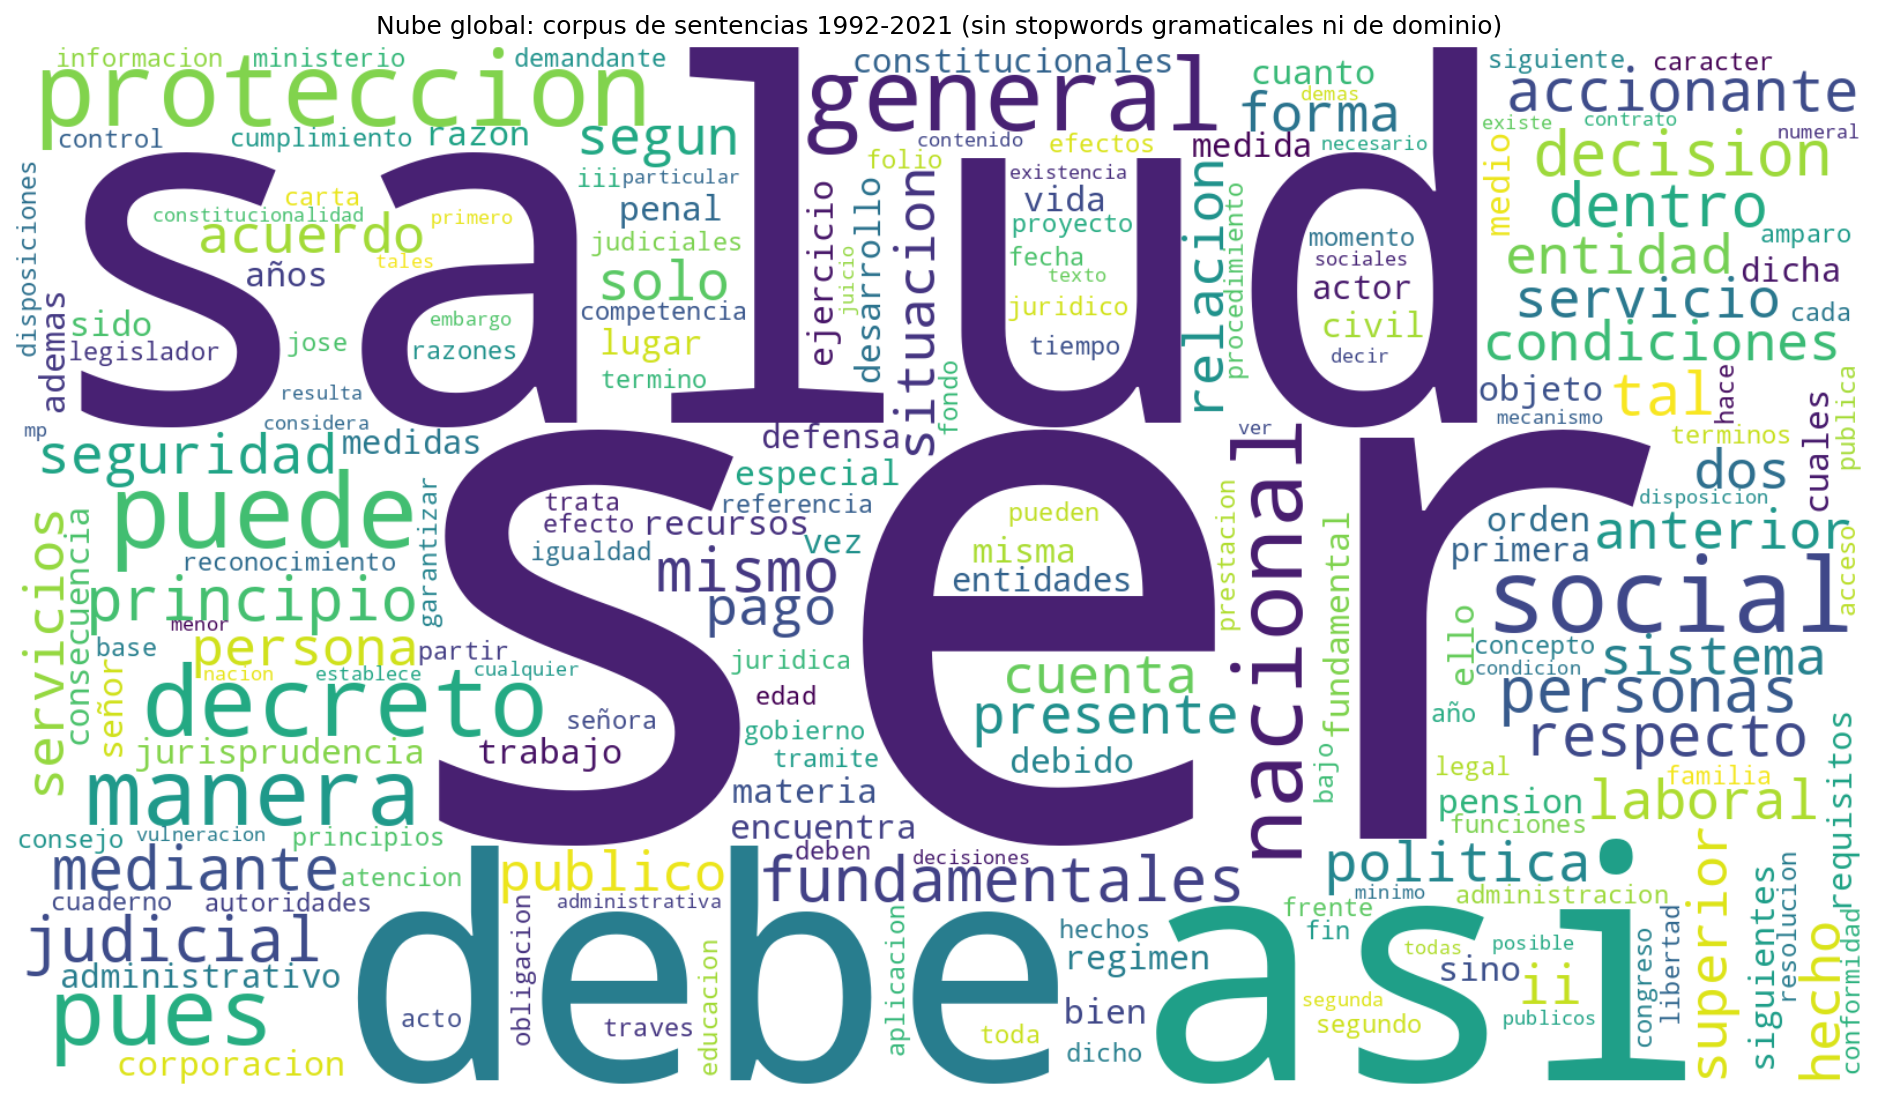
\includegraphics[width=0.55\linewidth]{fig_nube_global.png}
    \caption{Nube global de contenido: términos más frecuentes tras retirar las palabras vacías gramaticales y 65 formas de vocabulario jurídico-procesal de género.}
    \label{fig:nube_global}
\end{figure}

\begin{figure}[htbp]
    \centering
    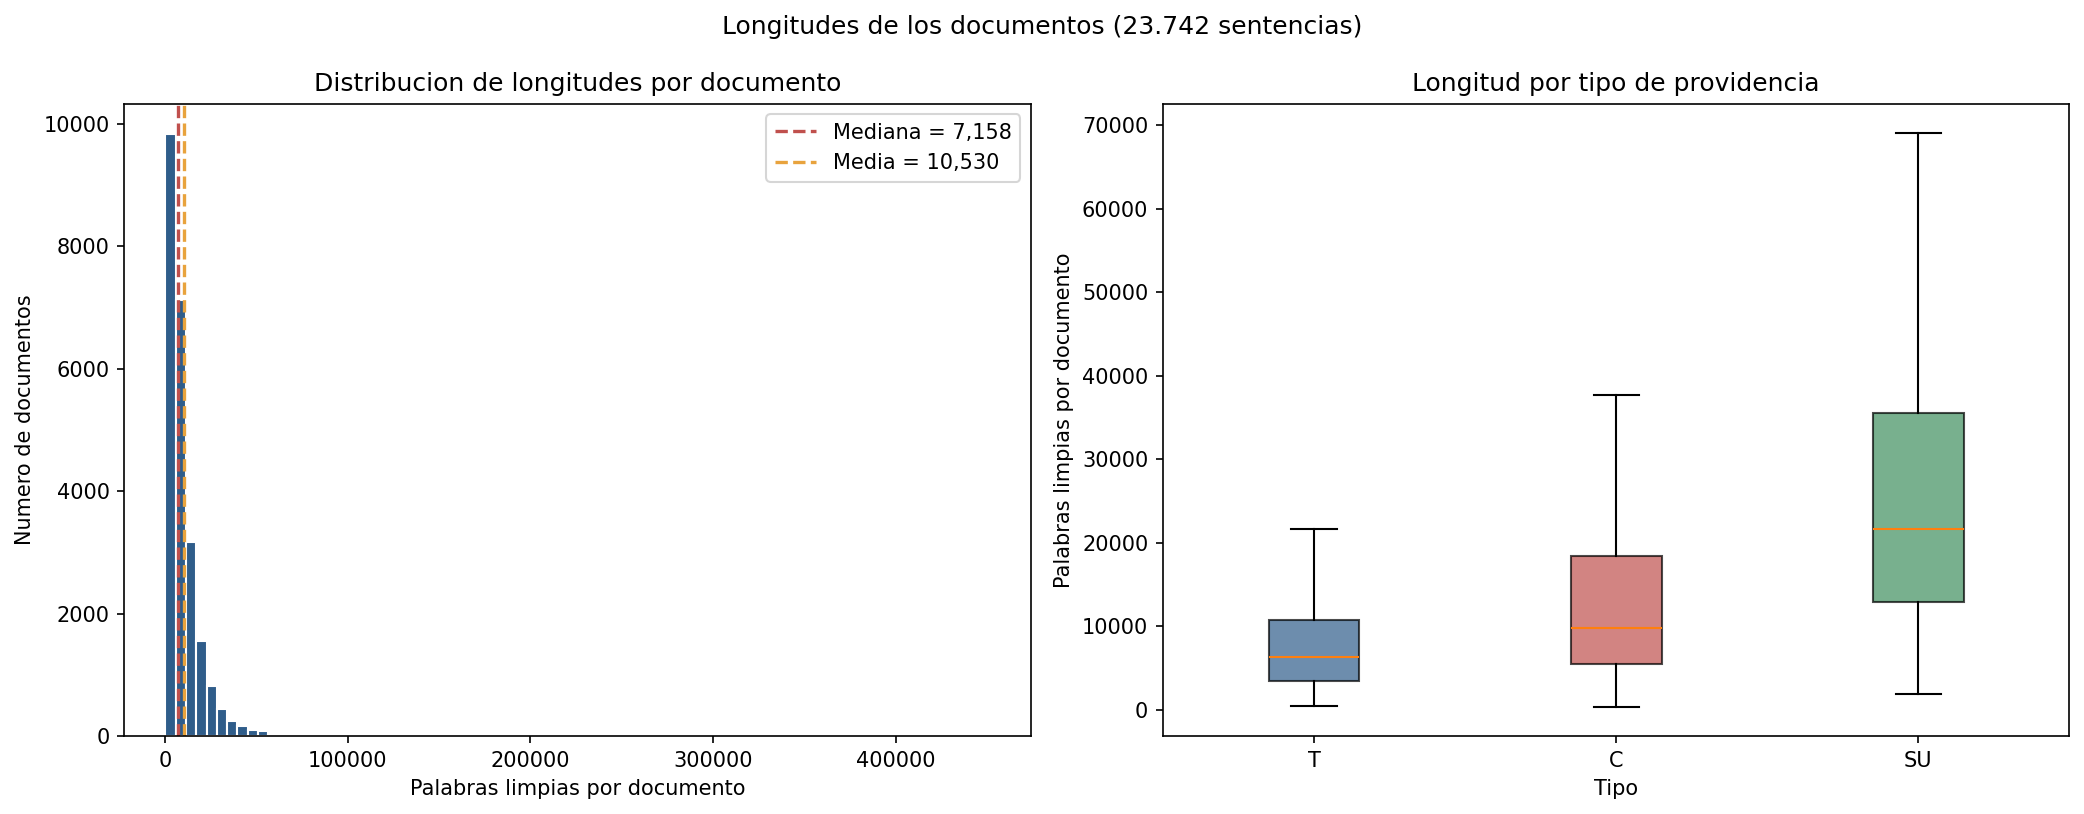
\includegraphics[width=0.88\linewidth]{fig_longitudes_documentos.png}
    \caption{Perfil de longitudes de los documentos (palabras limpias): distribución global con mediana y media (izquierda) y caja por tipo de providencia, sin valores atípicos (derecha).}
    \label{fig:longitudes}
\end{figure}

\begin{figure}[htbp]
    \centering
    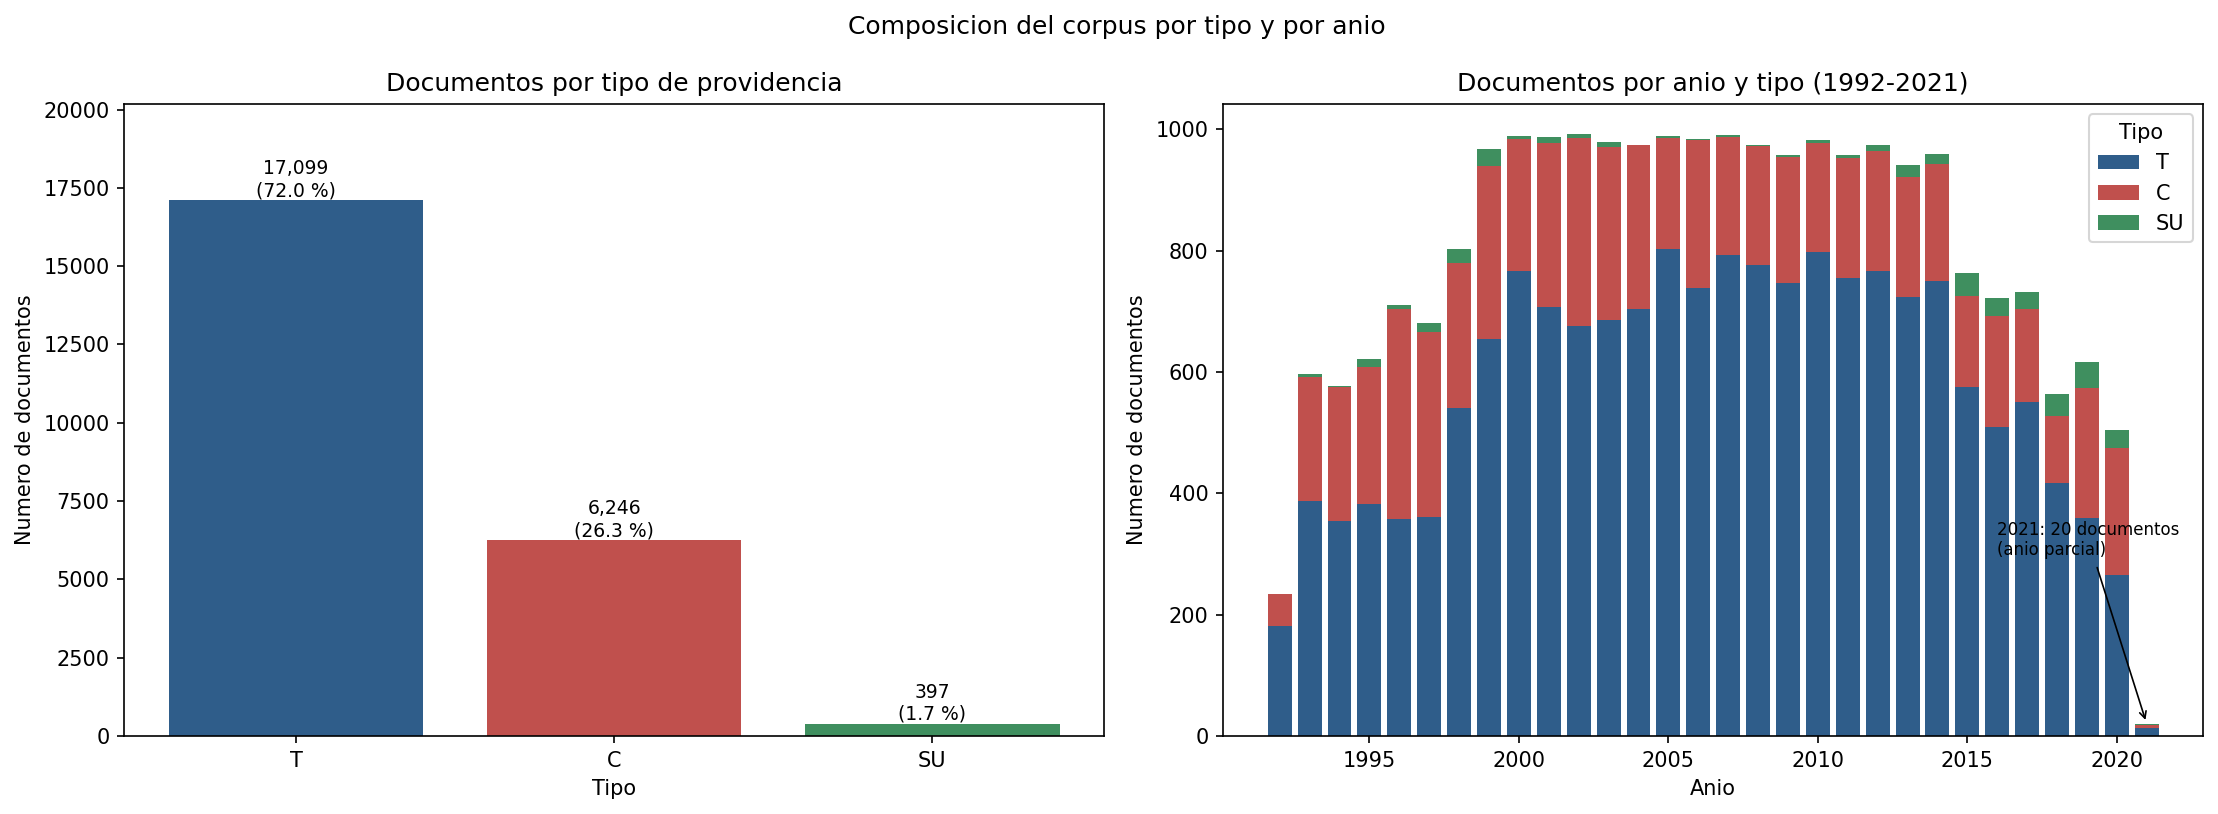
\includegraphics[width=0.92\linewidth]{fig_tipos_por_anio.png}
    \caption{Composición del corpus por tipo de providencia: totales y porcentajes (izquierda) y evolución anual apilada 1992--2021 (derecha); el bloque de 2021 corresponde a un año parcial (20 documentos).}
    \label{fig:tipos}
\end{figure}

% =====================================================================
% SECCION 4: EDA AVANZADO
% =====================================================================
\section{Análisis exploratorio avanzado}
\label{sec:eda}

Esta sección desarrolla el requisito 2 del enunciado. Todos los análisis se ejecutaron sobre el corpus completo y sus resultados quedan disponibles en \texttt{resultados/} y su subcarpeta \texttt{eda\_extendido/} (archivos CSV, Markdown y \emph{parquet} citados en cada subsección), de modo que cada cifra reportada aquí es trazable a un artefacto reproducible.

\subsection{N-gramas y colocaciones}
\label{sec:ngramas}
El análisis de n-gramas se ejecutó en una pasada por \emph{streaming} sobre el texto limpio de los 23.742 documentos, con dos reglas de filtrado: los bigramas se conservan solo si ambos extremos son palabras de contenido (sin palabras vacías); los trigramas se conservan con el mismo criterio y se marcan como fórmula (\texttt{es\_formula}) cuando la palabra intermedia es vacía, patrón típico de las fórmulas jurídicas del tipo \emph{accion de tutela} o \emph{proyecto de ley}. Se guardaron los 20.000 n-gramas más frecuentes de cada orden con poda periódica de hápax (los conteos altos quedan exactos). De los 20.000 trigramas guardados, 16.543 (82,7\,\%) presentan la palabra intermedia vacía, lo que confirma el carácter formulaico del género.

La tabla \ref{tab:ngramas} muestra los diez bigramas y trigramas más frecuentes. Los bigramas combinan conceptos doctrinales (\emph{derechos fundamentales}, 241.467; \emph{seguridad social}, 131.119; \emph{debido proceso}, 105.395; \emph{minimo vital}, 63.487) con sintagmas procesales (\emph{corte constitucional}, 286.786; \emph{primera instancia}, 65.203). Los trigramas están dominados por el mecanismo de amparo: \emph{accion de tutela} (344.893) supera en frecuencia a cualquier otro n-grama de contenido del corpus, lo que refleja que las tutelas representan el 72,02\,\% de los documentos. Aparecen también fórmulas de cita normativa (\emph{articulo del decreto}, 89.352; \emph{articulo del codigo}, 38.620), institucionales (\emph{suprema de justicia}, 50.638; \emph{sala de casacion}) y nombres de magistrados citados con insistencia (\emph{manuel jose cepeda}, 33.071), que la validación manual clasificó como entidades y no como fórmulas temáticas.

La distribución de frecuencias que sostiene estas listas se cuantifica en la figura \ref{fig:zipf}. Sobre los 20.000 unigramas más frecuentes del corpus, la relación entre rango y frecuencia en escala logarítmica es prácticamente lineal, con pendiente ajustada de $-1,4676$ y $R^2 = 0,9717$; los cinco términos de mayor rango son \emph{de}, \emph{la}, \emph{el}, \emph{que} y \emph{en}, los mismos que encabezan el top-20 del corpus (figura \ref{fig:top20}). En una gráfica log-log, una relación potencial se lee como una recta, de modo que el ajuste indica que las frecuencias del corpus siguen de cerca la ley de Zipf: unas pocas formas concentran la masa de ocurrencias y el resto decae de manera regular. Esta regularidad respalda las decisiones de vocabulario de la representación final ---frecuencia documental mínima de 3, recorte a 100.000 rasgos y ponderación sublineal--- documentadas en la sección \ref{sec:decision}.

\begin{table}[htbp]
    \centering
    \caption{Diez bigramas y diez trigramas más frecuentes del corpus (texto limpio; bigramas con extremos de contenido).}
    \label{tab:ngramas}
    \begin{tabular}{lr@{\hskip 0.6cm}lr}
        \toprule
        \multicolumn{2}{c}{\textbf{Bigramas}} & \multicolumn{2}{c}{\textbf{Trigramas}} \\
        \cmidrule(r){1-2}\cmidrule(l){3-4}
        \textbf{n-grama} & \textbf{frec.} & \textbf{n-grama} & \textbf{frec.} \\
        \midrule
        corte constitucional & 286.786 & accion de tutela & 344.893 \\
        derechos fundamentales & 241.467 & articulo del decreto & 89.352 \\
        seguridad social & 131.119 & suprema de justicia & 50.638 \\
        derecho fundamental & 111.146 & proyecto de ley & 43.384 \\
        constitucion politica & 109.220 & juez de tutela & 42.253 \\
        debido proceso & 105.395 & corte constitucional sentencia & 38.645 \\
        primera instancia & 65.203 & articulo del codigo & 38.620 \\
        minimo vital & 63.487 & administracion de justicia & 36.178 \\
        caso concreto & 63.089 & derecho de peticion & 34.429 \\
        debe ser & 62.378 & manuel jose cepeda & 33.071 \\
        \bottomrule
    \end{tabular}
\end{table}

Para decidir qué medida de asociación usar en las fases posteriores, se compararon tres criterios de ordenamiento de colocaciones ---frecuencia cruda, información mutua puntual (PMI) y razón de verosimilitud (LLR)--- sobre 20 casos evaluados manualmente (10 bigramas y 10 trigramas). La tabla \ref{tab:validacion} resume el veredicto: la frecuencia cruda alcanza un 55\,\% de fórmulas válidas, el PMI un 0\,\% y la LLR un 75\,\%. El PMI, al favorecer asociaciones raras de bajo soporte, ordena fragmentos ruidosos y no españoles (por ejemplo, \emph{aquaria eaza}, \emph{capromyidae capromys} o cadenas de caracteres), mientras que la frecuencia cruda rescata plantillas institucionales y nombres propios frecuentes pero arrastra combinaciones genéricas (\emph{debe ser}, \emph{primera instancia}). La razón de verosimilitud, en cambio, equilibra frecuencia y asociación y concentra fórmulas de dominio \cite{dunning1993accurate}; por ello se adopta como medida principal para las fases de modelado y recuperación. La figura \ref{fig:ngramas} muestra el top-15 de bi y trigramas, y la figura \ref{fig:colocaciones} el top-10 de colocaciones por LLR, donde destacan \emph{derechos fundamentales} y \emph{corte constitucional} en bigramas y \emph{accion de tutela} en trigramas.

\begin{table}[htbp]
    \centering
    \caption{Validación manual de 20 colocaciones (10 bigramas y 10 trigramas): porcentaje de fórmulas jurídicas válidas por medida.}
    \label{tab:validacion}
    \begin{tabular}{lccc}
        \toprule
        \textbf{Medida} & \textbf{Bigramas} & \textbf{Trigramas} & \textbf{Promedio} \\
        \midrule
        Frecuencia & 55\,\% & 55\,\% & 55\,\% \\
        PMI & 0\,\% & 0\,\% & 0\,\% \\
        Razón de verosimilitud (LLR) & 50\,\% & 100\,\% & 75\,\% \\
        \bottomrule
    \end{tabular}
\end{table}

\begin{figure}[htbp]
    \centering
    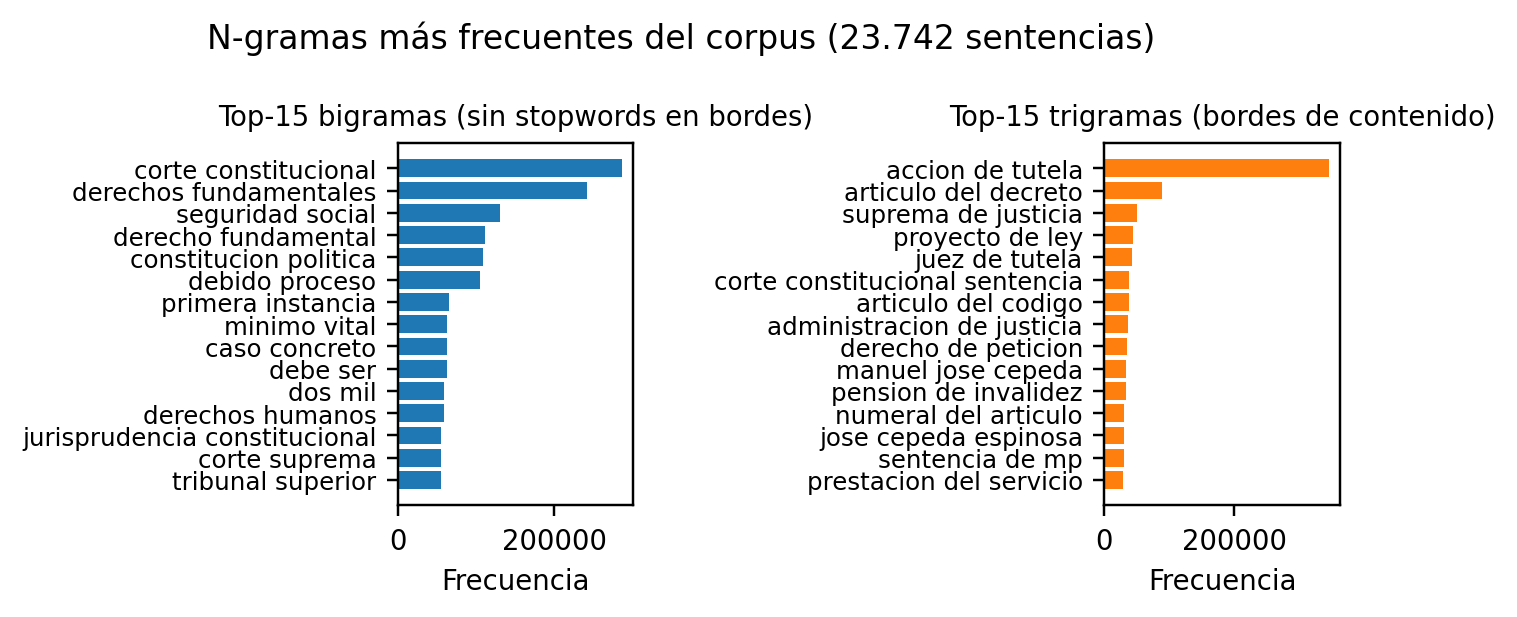
\includegraphics[width=0.78\linewidth]{fig_ngramas_bi_tri.png}
    \caption{Top-15 de bigramas y trigramas más frecuentes del corpus.}
    \label{fig:ngramas}
\end{figure}

\begin{figure}[htbp]
    \centering
    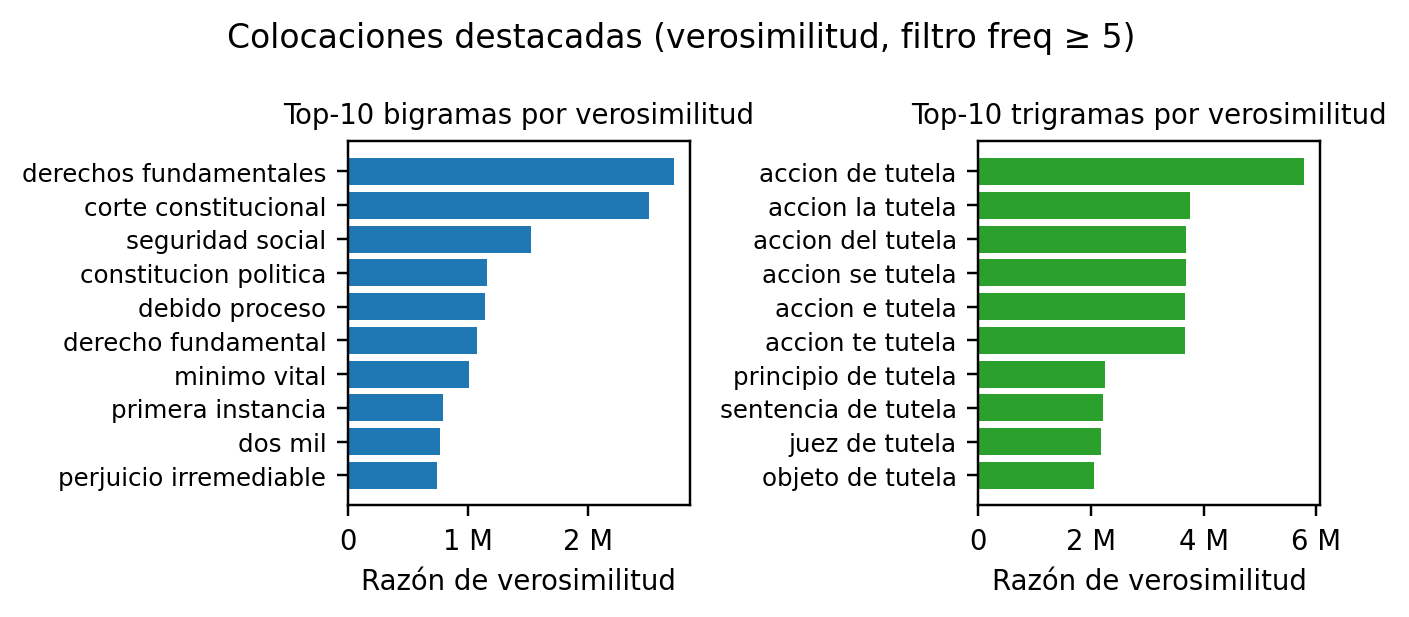
\includegraphics[width=0.78\linewidth]{fig_colocaciones.png}
    \caption{Colocaciones destacadas por razón de verosimilitud (filtro de frecuencia $\geq$ 5): top-10 de bigramas y de trigramas.}
    \label{fig:colocaciones}
\end{figure}

\begin{figure}[htbp]
    \centering
    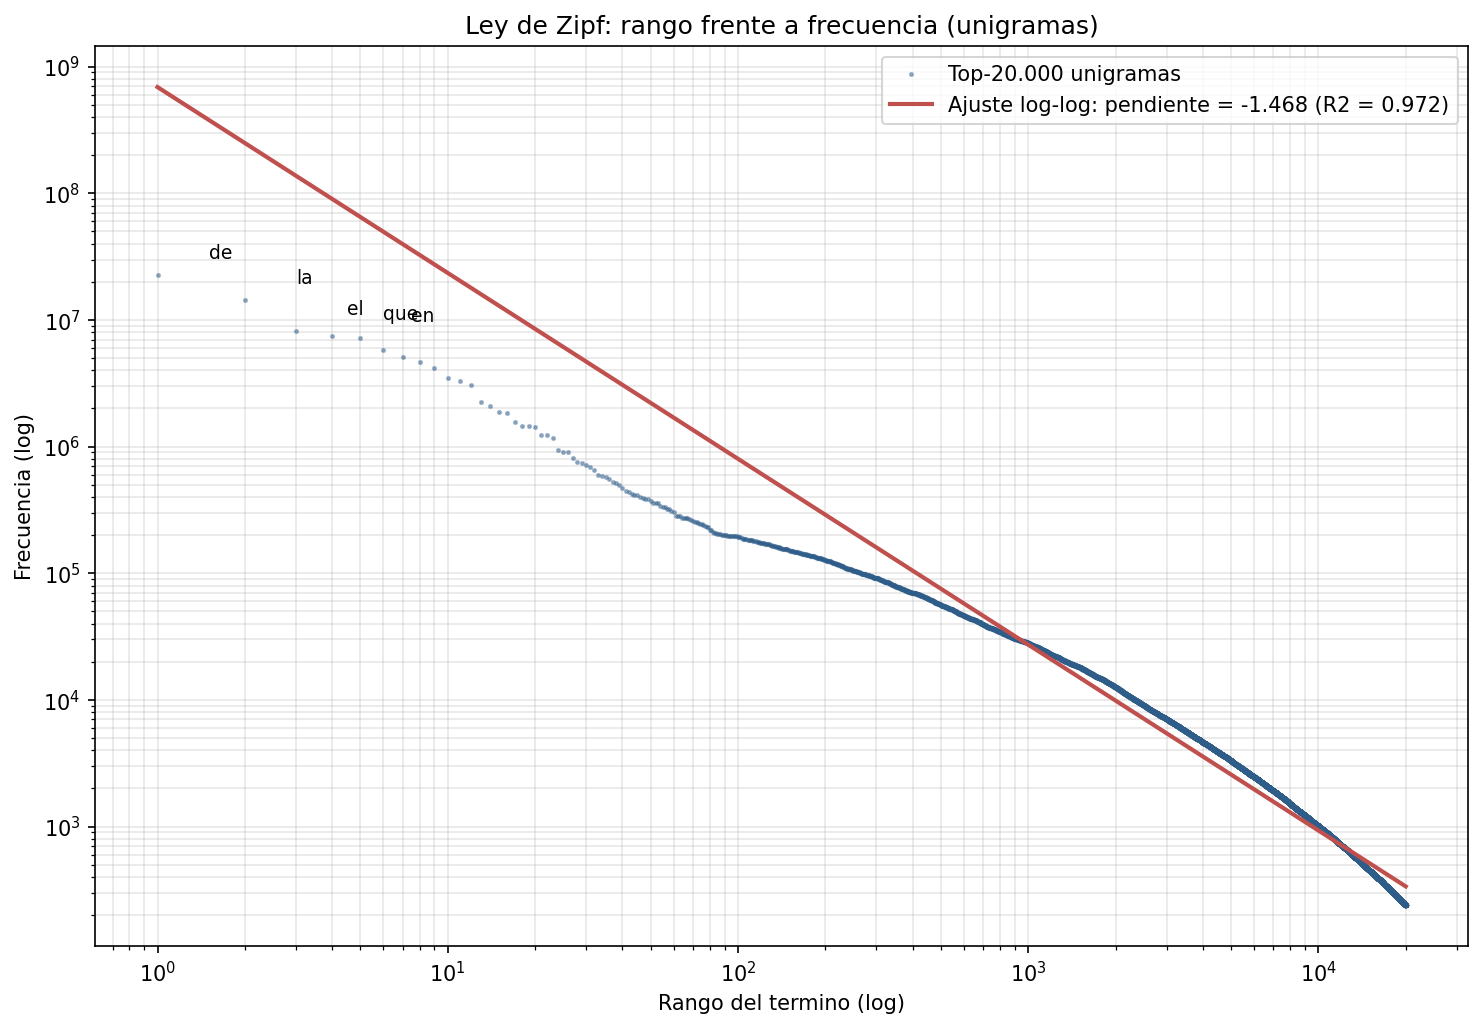
\includegraphics[width=0.62\linewidth]{fig_zipf.png}
    \caption{Ley de Zipf sobre el top-20.000 de unigramas del corpus: rango frente a frecuencia en escala logarítmica y ajuste lineal (pendiente $-1,4676$; $R^2 = 0,9717$).}
    \label{fig:zipf}
\end{figure}

\subsection{Diversidad léxica: MTLD}
\label{sec:mtld}
La diversidad léxica se midió con MTLD (\emph{Measure of Textual Lexical Diversity}), una medida robusta frente a la longitud del texto a diferencia del TTR crudo \cite{mccarthy2010mtld}. El algoritmo recorre el documento acumulando TTR y cuenta un factor cada vez que el TTR cae al umbral de 0,72; la MTLD final es la media bidireccional de tokens por factor. El cálculo se hizo por documento sobre los tokens alfabéticos de la pasada morfológica. La MTLD media global es de 61,03 (mediana 60,69; mínimo 25,80; máximo 114,12) y la tabla \ref{tab:mtld} la desglosa por tipo de providencia y por periodo.

\begin{table}[htbp]
    \centering
    \caption{MTLD por tipo de providencia y por periodo (umbral 0,72).}
    \label{tab:mtld}
    \begin{tabular}{lrrr}
        \toprule
        \textbf{Grupo} & \textbf{Media} & \textbf{Mediana} & \textbf{Documentos} \\
        \midrule
        Global & 61,03 & 60,69 & 23.742 \\
        T (tutela) & 61,63 & 61,21 & 17.099 \\
        C (constitucionalidad) & 59,54 & 59,43 & 6.246 \\
        SU (unificación) & 58,88 & 58,72 & 397 \\
        \midrule
        1992--2001 & 64,32 & 64,09 & 7.166 \\
        2002--2011 & 60,37 & 60,19 & 9.779 \\
        2012--2021 & 58,53 & 58,32 & 6.797 \\
        \bottomrule
    \end{tabular}
\end{table}

Tres lecturas se desprenden de la tabla. Primero, las tutelas son más diversas léxicamente (61,63) que las sentencias de constitucionalidad (59,54) y de unificación (58,88); una explicación plausible es que las tutelas narran casos individuales heterogéneos, mientras que las C y SU se apoyan más en plantillas doctrinales. Segundo, la diversidad desciende de forma sostenida a lo largo de las tres décadas: de 64,32 en 1992--2001 a 58,53 en 2012--2021. La regresión lineal sobre los 23.742 documentos estima una pendiente de $-0,32$ puntos de MTLD por año (correlación de Pearson $r = -0,328$, $p < 0,001$; Spearman $\rho = -0,330$), con medias anuales que pasan de $\approx$ 65,0 en 1992--1998 (promedio de las medias anuales del periodo) a 55,69 en 2020. Tercero, el patrón es consistente en los tres tipos de providencia, lo que sugiere un fenómeno de estandarización del estilo de redacción de la Corte más que un efecto de composición entre tipos. La figura \ref{fig:mtld} ilustra ambas dimensiones. Estas tendencias son descriptivas: la sección \ref{sec:periodos} las complementa con el contraste léxico por periodos.

\begin{figure}[htbp]
    \centering
    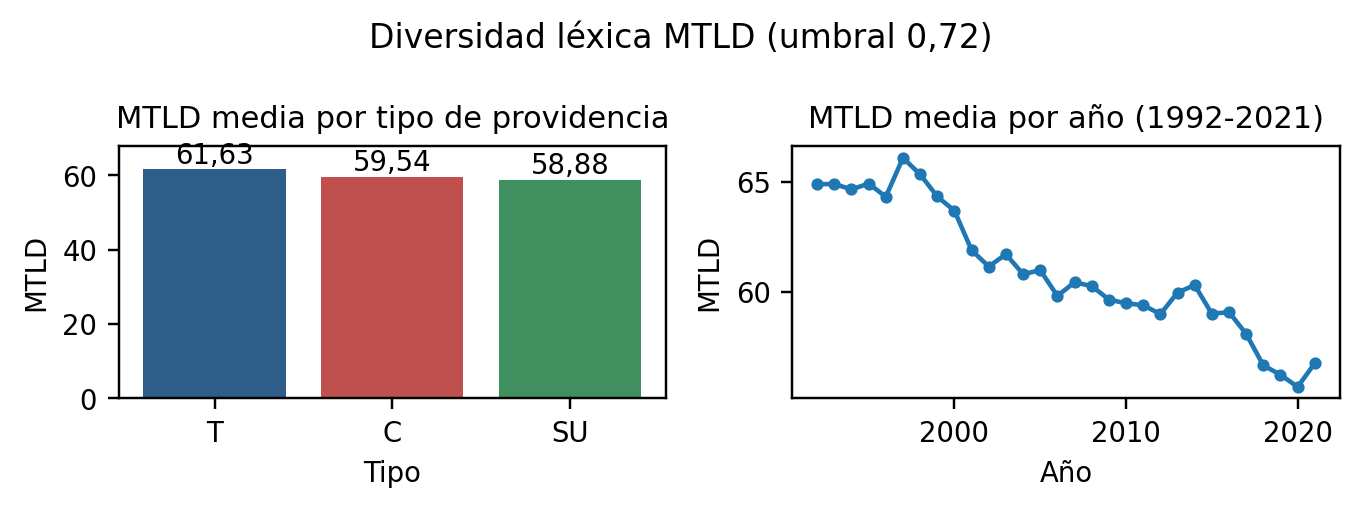
\includegraphics[width=0.78\linewidth]{fig_mtld_distribucion.png}
    \caption{Diversidad léxica MTLD: media por tipo de providencia (izquierda) y evolución de la media anual, 1992--2021 (derecha).}
    \label{fig:mtld}
\end{figure}

Una propiedad crítica de las medidas de diversidad es su estabilidad frente a la longitud del texto. La figura \ref{fig:mtld_longitud} verifica esa propiedad sobre los 23.742 documentos: el mapa de densidad (\emph{hexbin}) muestra la nube de documentos con el eje de tokens en escala logarítmica (rango observado: 314--449.822 tokens) y la línea roja resume la mediana de MTLD por intervalo logarítmico de longitud, lo que permite leer la tendencia central sin el peso visual de las zonas más densas. La asociación entre MTLD y longitud, medida con la correlación de Spearman, es débil y negativa ($\rho = -0,2628$): el tamaño del documento no domina la diversidad calculada, lo que respalda el uso de MTLD para comparar documentos de tamaños muy dispares (figura \ref{fig:longitudes}) y sostiene las lecturas por tipo y por periodo de la tabla \ref{tab:mtld}.

\begin{figure}[htbp]
    \centering
    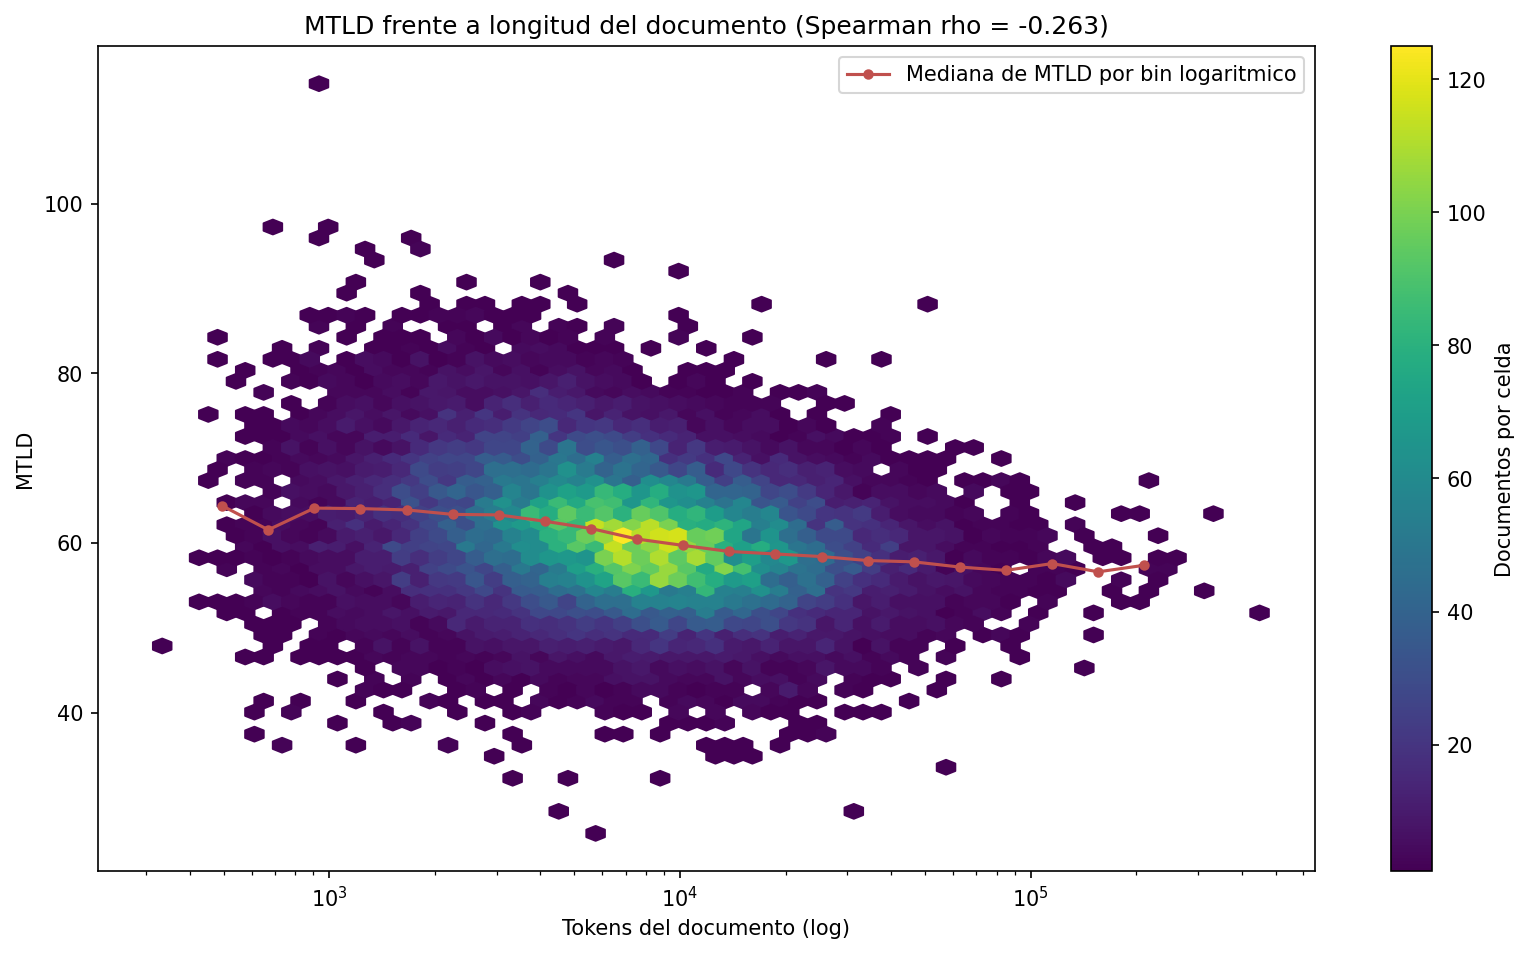
\includegraphics[width=0.62\linewidth]{fig_mtld_vs_longitud.png}
    \caption{MTLD frente a la longitud del documento: densidad de los 23.742 documentos (\emph{hexbin}, tokens en escala logarítmica) y mediana de MTLD por intervalo logarítmico; Spearman $\rho = -0,2628$.}
    \label{fig:mtld_longitud}
\end{figure}

\subsection{Morfología: lemas, \emph{stems} y categorías gramaticales}
\label{sec:morfologia}
La pasada morfológica se ejecutó sobre los 23.742 documentos con el modelo de spaCy para español \texttt{es\_core\_news\_md} ($\approx$ 87 minutos) y una pasada adicional de \emph{stemming} Snowball en español ($\approx$ 20 minutos). La tabla \ref{tab:morfologia} resume el efecto de cada representación sobre el vocabulario. La lematización reduce el vocabulario de formas en un 12,7\,\% (de 224.468 a 195.959 tipos) y agrupa flexiones que la forma superficial separa (\emph{derechos} y \emph{derecho} $\rightarrow$ \emph{derecho}; \emph{sentencias} $\rightarrow$ \emph{sentencia}); el \emph{stemming} lo reduce un 45,8\,\% (121.696 tipos), a costa de formas menos legibles (\emph{derecho} $\rightarrow$ \emph{derech}; \emph{corte} $\rightarrow$ \emph{cort}) que pueden fusionar términos distintos. La muestra de calidad de la pasada (lema y \emph{stem} de los tokens más frecuentes) se conserva en \texttt{lemas\_stems\_pos/muestra\_calidad.csv}.

\begin{table}[htbp]
    \centering
    \caption{Tamaño del vocabulario según la representación morfológica (23.742 documentos).}
    \label{tab:morfologia}
    \begin{tabular}{lrrl}
        \toprule
        \textbf{Representación} & \textbf{Vocabulario} & \textbf{\% del vocabulario de formas} & \textbf{Ejemplo} \\
        \midrule
        Formas (tokens) & 224.468 & 100\,\% & \emph{derechos} \\
        Lemas & 195.959 & 87,3\,\% & \emph{derecho} \\
        \emph{Stems} & 121.696 & 54,2\,\% & \emph{derech} \\
        \bottomrule
    \end{tabular}
\end{table}

La distribución de categorías gramaticales (POS) es estable y coherente con el registro jurídico: NOUN (22,58\,\%), ADP (20,45\,\%), DET (15,57\,\%), ADJ (9,15\,\%), PROPN (8,32\,\%) y VERB (7,94\,\%) encabezan el conteo global. Por tipo de providencia las diferencias son de pocas décimas: las C presentan algo más de adjetivos (9,47\,\% frente a 8,96\,\% en T) y algo menos de nombres propios (7,67\,\% frente a 8,70\,\% en T), consistente con un discurso más doctrinal y menos narrativo; las T y SU son casi idénticas entre sí. Las figuras \ref{fig:lemmastem} y \ref{fig:pos} ilustran la compresión de vocabulario y la distribución POS global y por tipo. En términos de representación, el resultado relevante es que la lematización ofrece una reducción de vocabulario apreciable manteniendo la legibilidad y la interpretabilidad de los rasgos, condición útil para una representación basada en pesos de términos (sección \ref{sec:decision}).

\begin{figure}[htbp]
    \centering
    \begin{subfigure}[t]{0.48\linewidth}
        \centering
        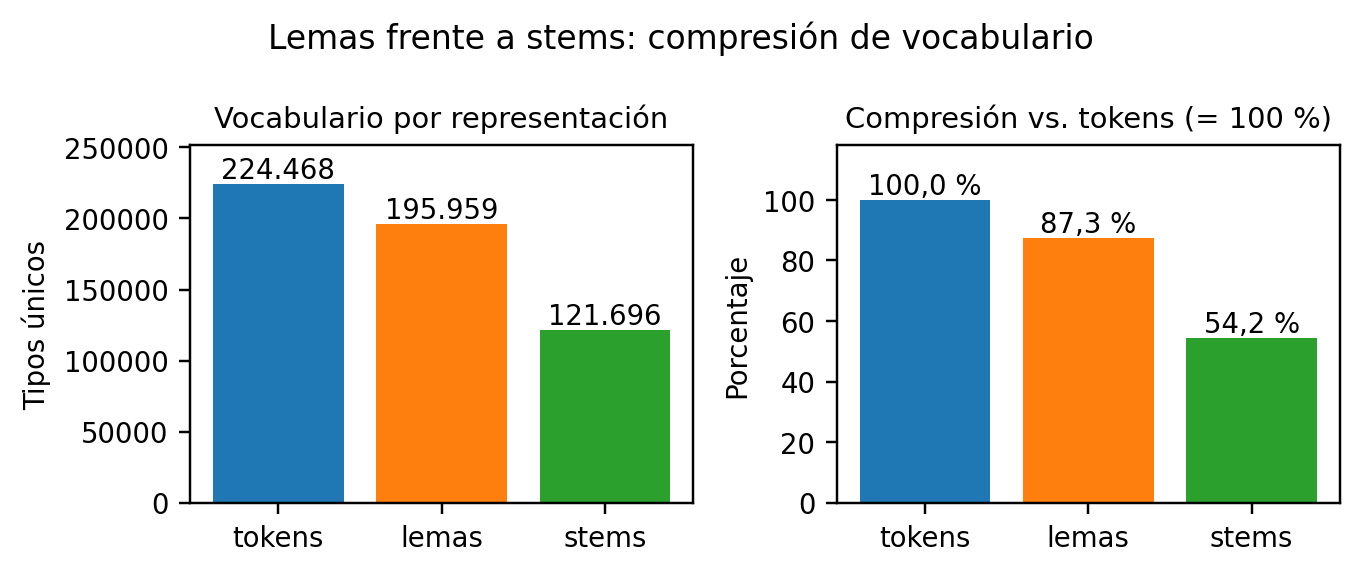
\includegraphics[width=\linewidth]{fig_lemma_vs_stem.png}
        \caption{Tamaño del vocabulario por representación (formas, lemas y \emph{stems}).}
        \label{fig:lemmastem}
    \end{subfigure}%
    \hfill
    \begin{subfigure}[t]{0.48\linewidth}
        \centering
        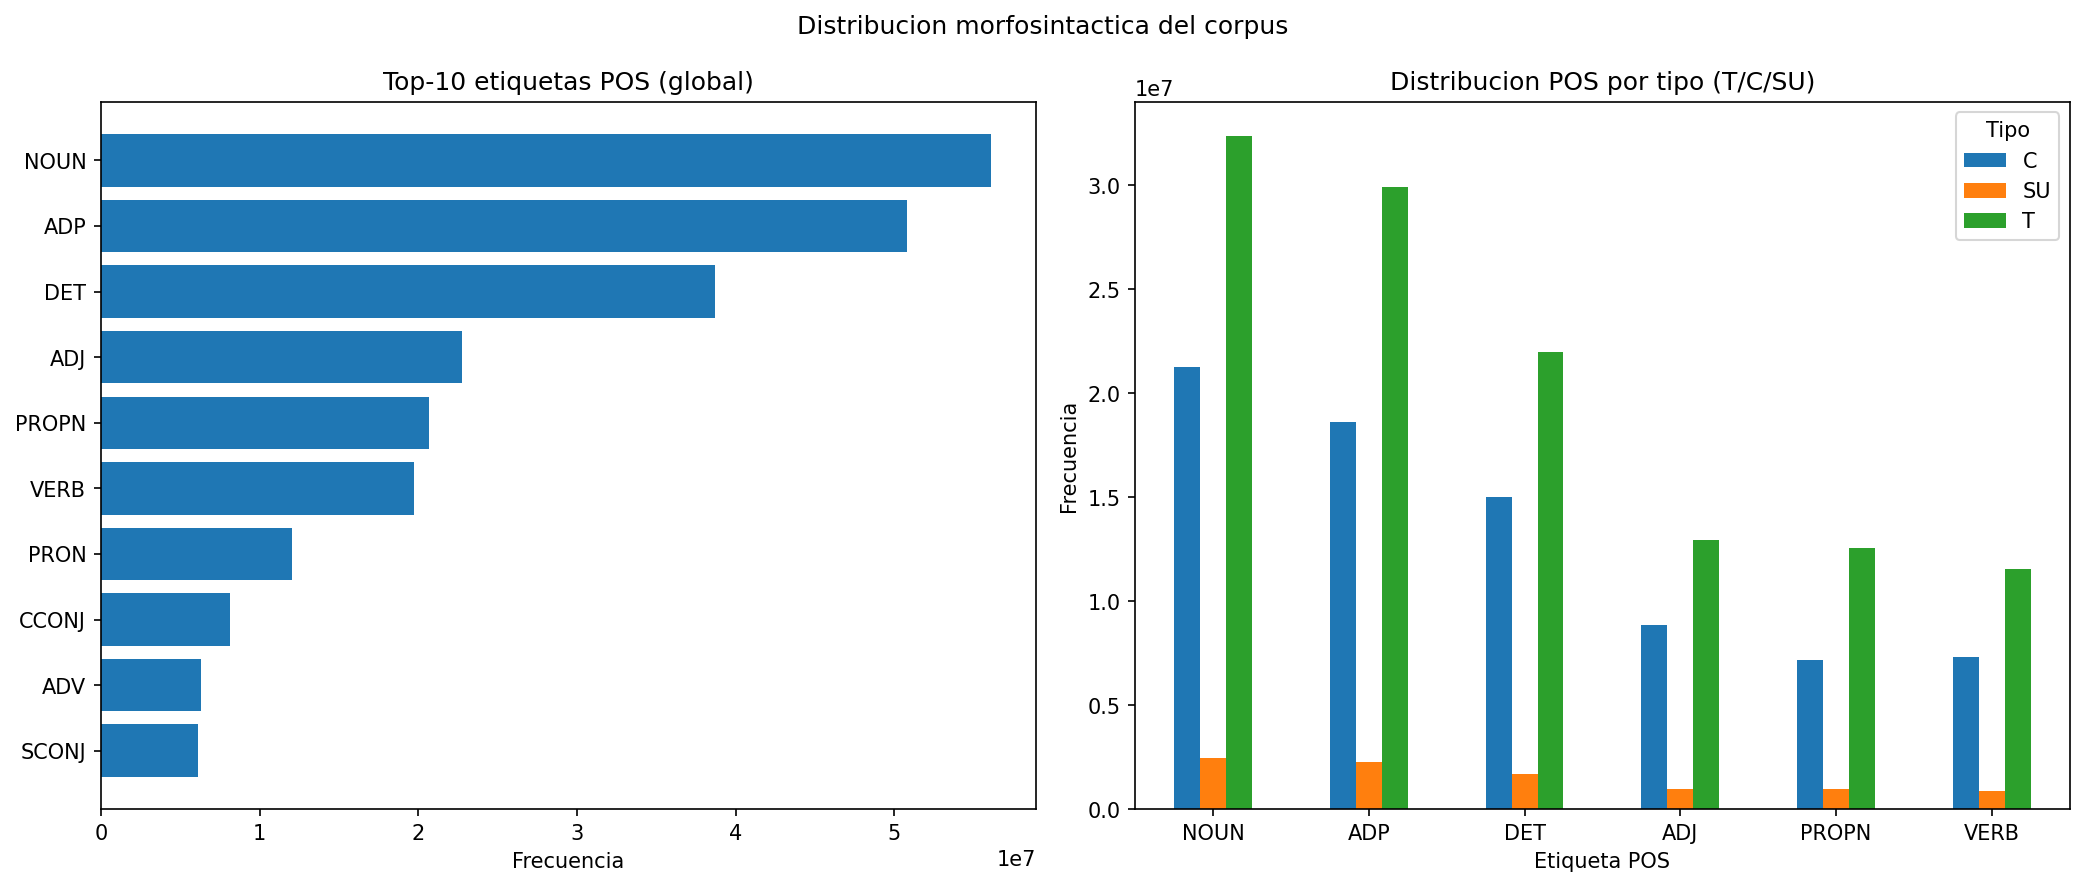
\includegraphics[width=\linewidth]{fig_pos_distribucion.png}
        \caption{Distribución de categorías gramaticales (POS).}
        \label{fig:pos}
    \end{subfigure}
    \caption{Evidencia morfológica: compresión del vocabulario por representación (izquierda) y distribución POS global y por tipo de providencia (derecha).}
\end{figure}

\subsection{Evolución léxica por periodos}
\label{sec:periodos}
La Entrega 1 prometió el análisis cuantitativo de la evolución léxica por periodos; esta subsección lo ejecuta y reporta. Se definen tres periodos de extensión comparable: 1992--2001 (7.166 documentos; 19.950.956 tokens-lema sin palabras vacías), 2002--2011 (9.779; 48.671.763) y 2012--2021 (6.797; 62.545.530; el año 2021 es parcial, con 20 documentos). El conteo se hizo sobre los lemas normalizados por documento (sección \ref{sec:dataset}), sin palabras vacías, y cubrió 192.277 formas únicas en 40,5 segundos. Para cada transición se ordenan los lemas por su razón de \emph{log-odds} binaria con suavizado add-0,5 \cite{hamilton2016diachronic}: para un lema $w$ y los periodos base $b$ y objetivo $t$,
\begin{equation}
\delta_w = \log\!\left(\frac{f_w^{t} + 0,5}{N_t - f_w^{t} + 0,5}\right) - \log\!\left(\frac{f_w^{b} + 0,5}{N_b - f_w^{b} + 0,5}\right),
\label{eq:logodds}
\end{equation}
donde $f_w^{b}$ y $f_w^{t}$ son las frecuencias del lema en cada periodo y $N_b$ y $N_t$ los totales de tokens-lema; solo se consideran lemas con frecuencia combinada $\geq$ 50, con la misma configuración del módulo de diacronía del proyecto. El signo es relativo: un lema que ``baja'' puede seguir siendo frecuente; lo que cambia es su peso relativo en el vocabulario del periodo. Este contraste es una práctica establecida para identificar el léxico distintivo entre subcorpus, incluido el análisis diacrónico de tribunales \cite{raj2026collective}. La tabla \ref{tab:logodds} muestra los diez lemas que más suben y más bajan en cada transición y la figura \ref{fig:logodds} ilustra la segunda; la tabla completa (42.362 filas) queda en \texttt{resultados/diacronia\_logodds.csv}.

\begin{table}[htbp]
    \centering
    \caption{Lemas con mayor cambio relativo entre periodos (log-odds con suavizado add-0,5; frecuencia combinada $\geq$ 50). Primera transición: 1992--2001 $\rightarrow$ 2002--2011; segunda: 2002--2011 $\rightarrow$ 2012--2021. Valores redondeados a una décima.}
    \label{tab:logodds}
    \small
    \begin{tabular}{cp{0.20\textwidth}p{0.20\textwidth}p{0.20\textwidth}p{0.20\textwidth}}
        \toprule
        \textbf{\#} & \textbf{Sube (1.\textsuperscript{a})} & \textbf{Baja (1.\textsuperscript{a})} & \textbf{Sube (2.\textsuperscript{a})} & \textbf{Baja (2.\textsuperscript{a})} \\
        \midrule
        1 & incoder (7,1) & juzg ($-$8,5) & uariv (9,2) & nilser ($-$6,5) \\
        2 & rupd (6,9) & trasladante ($-$6,7) & jep (9,0) & fomin ($-$6,2) \\
        3 & chaljub (6,7) & sgpc ($-$6,3) & coronavirus (9,0) & superview ($-$6,0) \\
        4 & fonvivienda (6,6) & indalpe ($-$6,2) & gnr (8,1) & sarai ($-$6,0) \\
        5 & cisa (6,4) & dcho ($-$6,2) & arl (7,9) & guingue ($-$5,9) \\
        6 & bariatrico (6,4) & obtentor ($-$6,2) & zidres (7,6) & serpvir ($-$5,8) \\
        7 & colmedica (6,3) & croydon ($-$6,0) & anla (7,5) & capruis ($-$5,8) \\
        8 & indiciado (6,3) & mecanizados ($-$5,9) & cgp (7,5) & intelsat ($-$5,8) \\
        9 & afrodescendient (6,2) & cuo ($-$5,9) & unp (7,5) & commsa ($-$5,8) \\
        10 & humanavivir (6,0) & clad ($-$5,8) & cev (7,3) & cja ($-$5,7) \\
        \bottomrule
    \end{tabular}
\end{table}

\textbf{Lectura.} En la primera transición (1992--2001 $\rightarrow$ 2002--2011) ganan peso siglas y nombres de entidades que reflejan nuevas materias y actores del periodo (\emph{incoder}, \emph{rupd}, \emph{fonvivienda}, \emph{cisa}, \emph{colmedica}, \emph{humanavivir}) y retroceden formas procesales y ruido de digitalización (\emph{juzg}, \emph{sgpc}, \emph{dcho}, \emph{indalpe}). En la segunda (2002--2011 $\rightarrow$ 2012--2021) el ascenso es nítidamente temático: \emph{uariv} (Unidad para las Víctimas), \emph{jep}, \emph{coronavirus}, \emph{arl}, \emph{zidres}, \emph{anla} y \emph{cgp}, vocabulario asociado al conflicto armado, la pandemia y la institucionalidad reciente, mientras descienden nombres propios y abreviaturas del periodo anterior (\emph{nilser}, \emph{fomin}, \emph{superview}, \emph{sarai}). Los resultados se interpretan como indicios temáticos (nuevas materias y cambios de lenguaje procesal), no como afirmaciones causales.

\begin{figure}[htbp]
    \centering
    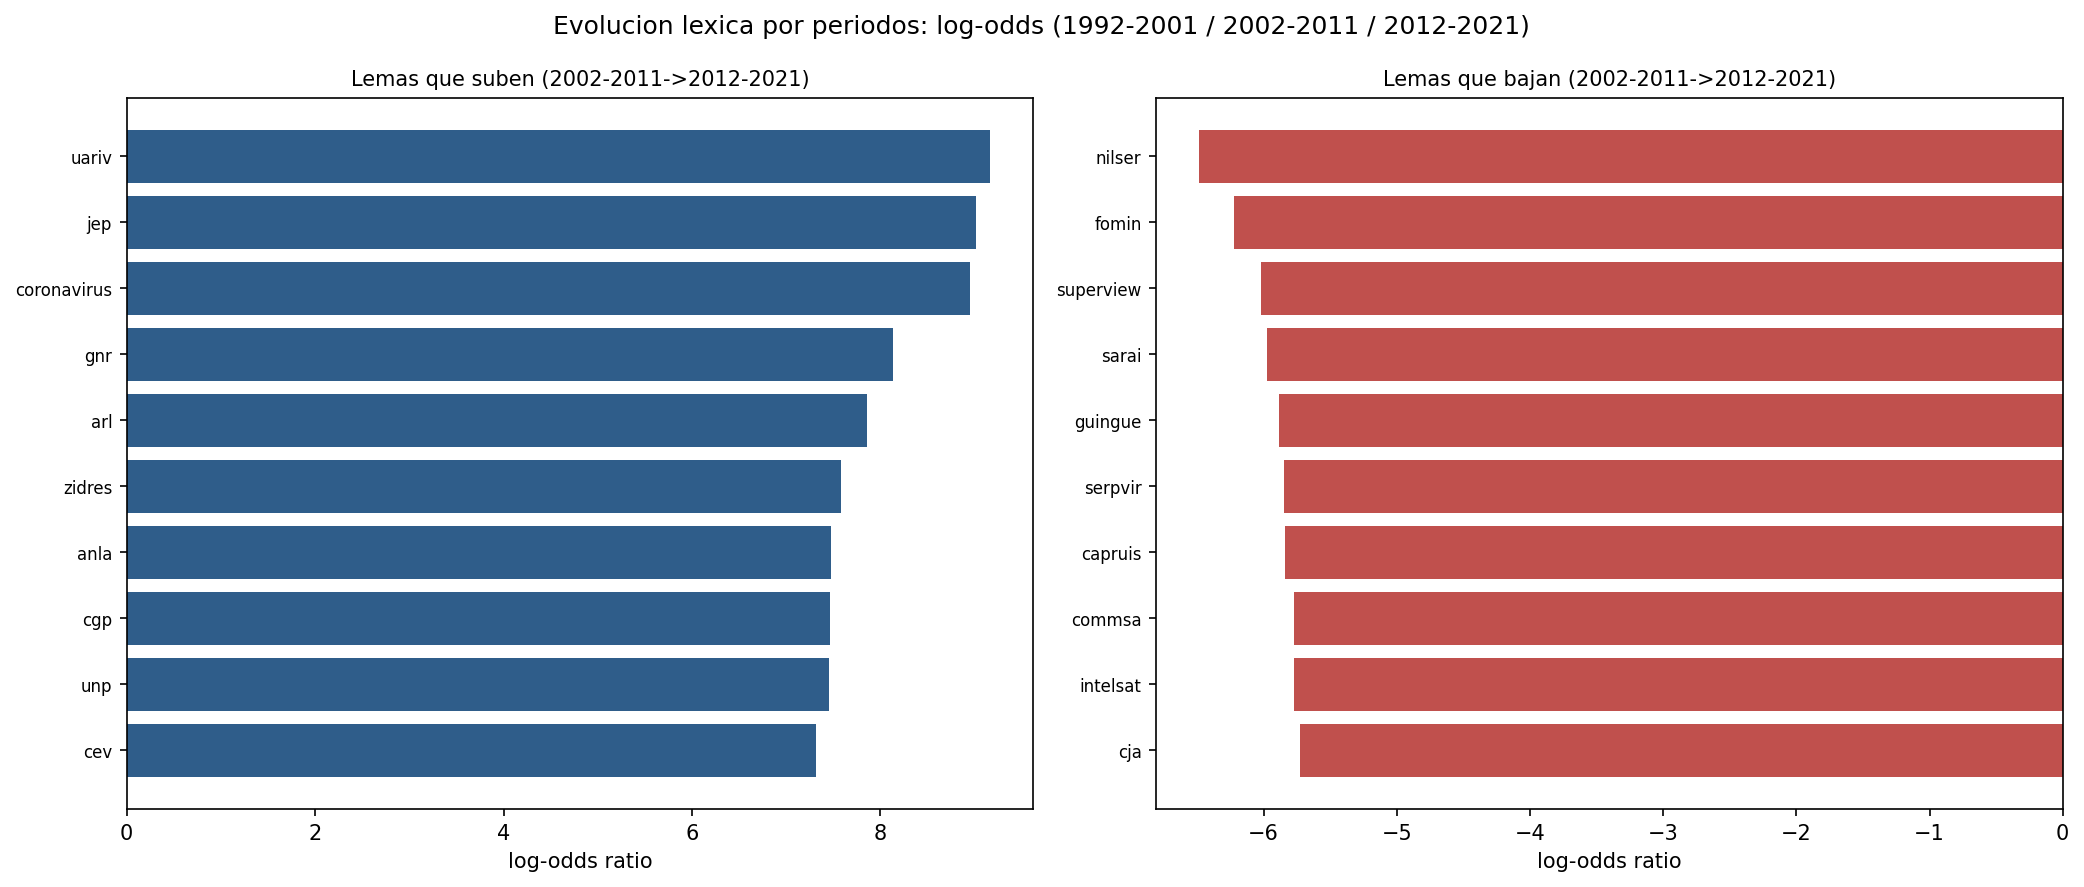
\includegraphics[width=0.68\linewidth]{fig_logodds_periodos.png}
    \caption{Evolución léxica por periodos: diez lemas con mayor log-odds positivo (izquierda) y negativo (derecha) en la transición 2002--2011 $\rightarrow$ 2012--2021.}
    \label{fig:logodds}
\end{figure}

\textbf{Limitación (datos conservados, no ocultos).} Los extremos de las listas incluyen siglas institucionales sin desarrollar, nombres propios y ruido de OCR/abreviaturas del corpus; el método replica la referencia interna del proyecto (mismos periodos, mismo suavizado y misma frecuencia mínima) y el solapamiento del top-10 con esa referencia es de 7/10 a 9/10 en las cuatro listas, con diferencias que provienen de la unidad de análisis (aquí lemas; en la referencia, formas superficiales) y de empates en el corte del top-10. La depuración de siglas y ruido de OCR, y la unificación de variantes, queda documentada como refinamiento para la fase de modelado y no se aplica aquí para no alterar el resultado reproducible del método estándar.

Como complemento cualitativo, la figura \ref{fig:nubes_periodos} conserva las nubes anuales de la Entrega 1 (tres paneles), que muestran la estabilidad de las fórmulas institucionales y la aparición de vocabulario temático propio de cada época; la serie de MTLD (sección \ref{sec:mtld}) aporta la tendencia cuantitativa global.

\begin{figure}[htbp]
    \centering
    \begin{subfigure}[b]{0.30\linewidth}
        \centering
        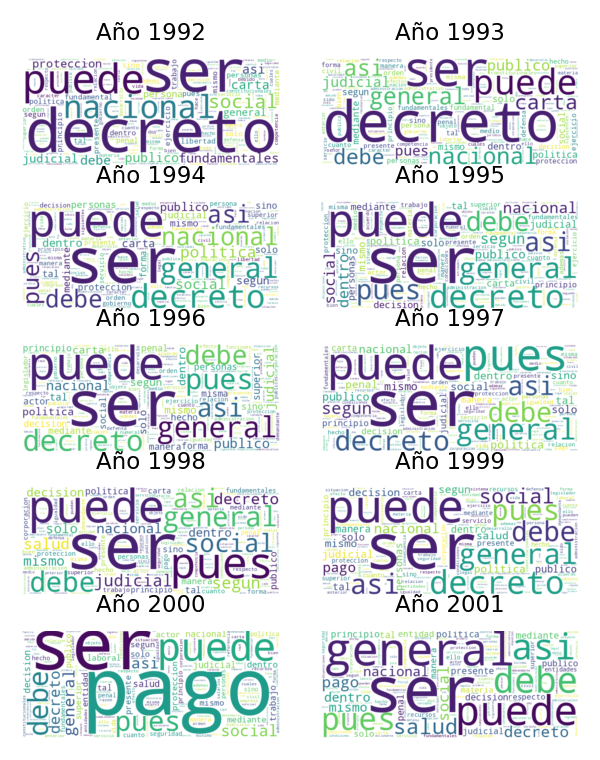
\includegraphics[width=\linewidth]{fig_nubes_por_anio_1992_2001.png}
        \caption{1992--2001.}
        \label{fig:nubes_p1}
    \end{subfigure}%
    \hfill
    \begin{subfigure}[b]{0.30\linewidth}
        \centering
        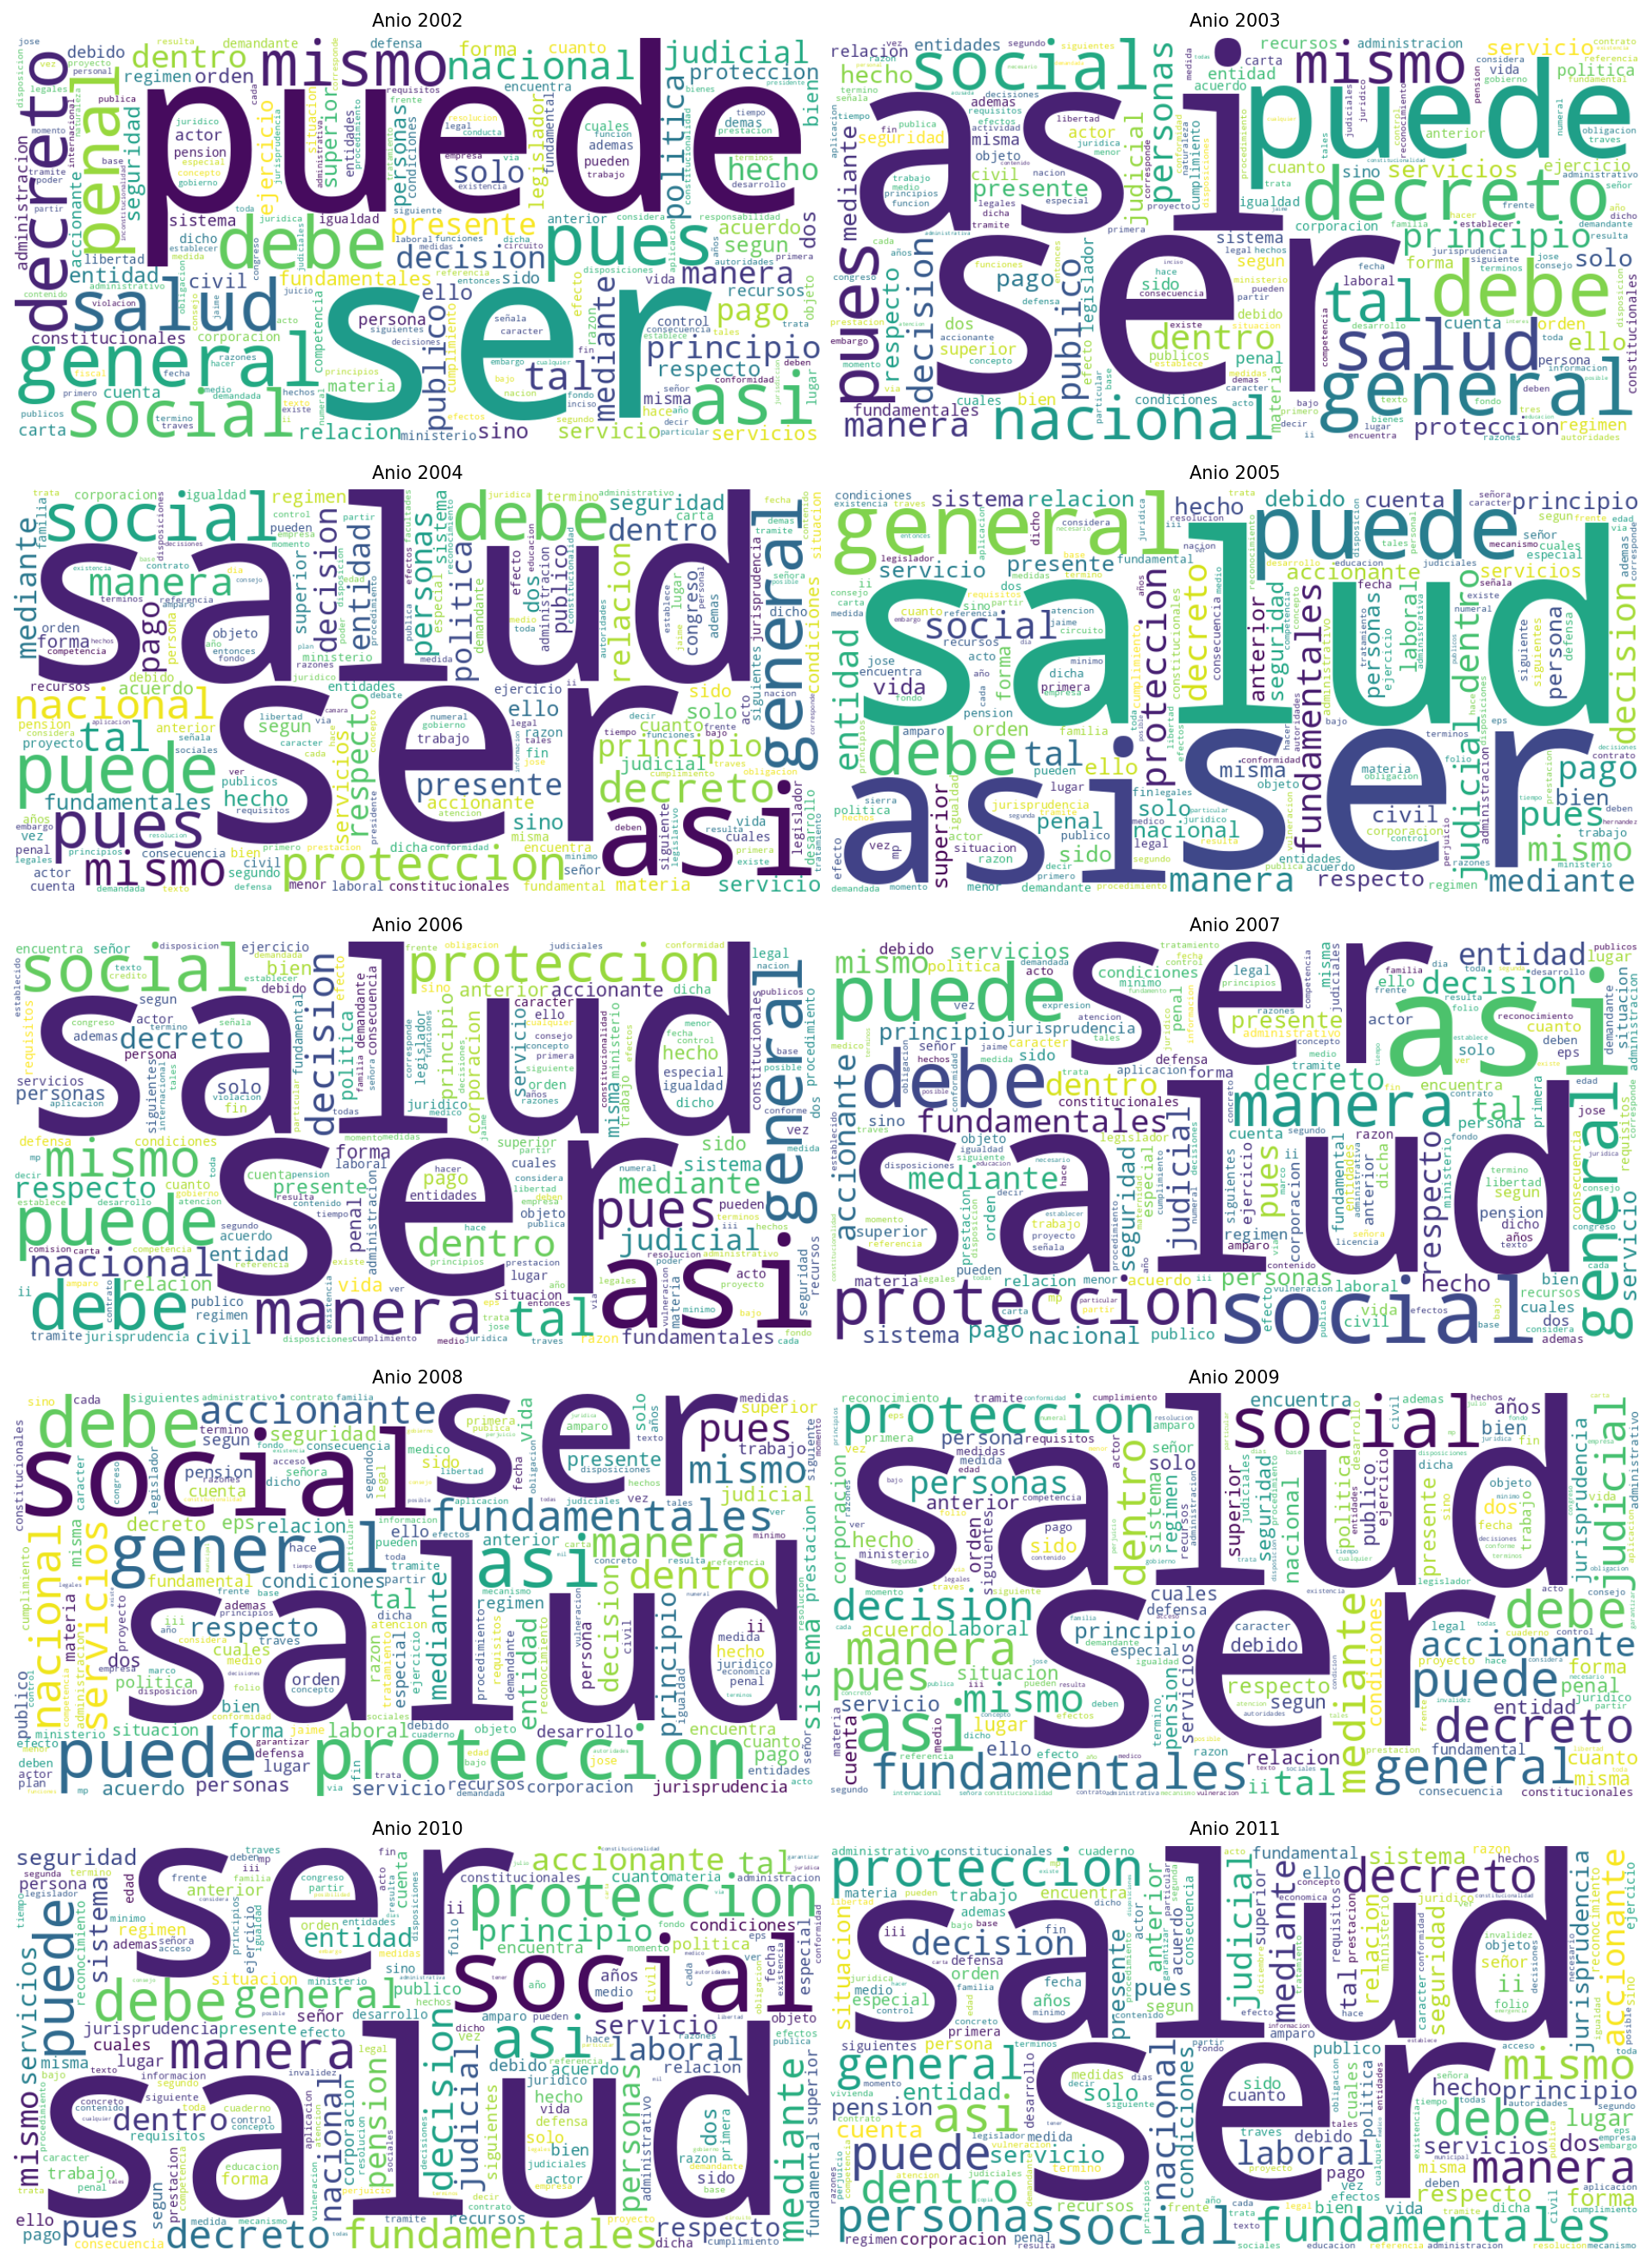
\includegraphics[width=\linewidth]{fig_nubes_por_anio_2002_2011.png}
        \caption{2002--2011.}
        \label{fig:nubes_p2}
    \end{subfigure}%
    \hfill
    \begin{subfigure}[b]{0.30\linewidth}
        \centering
        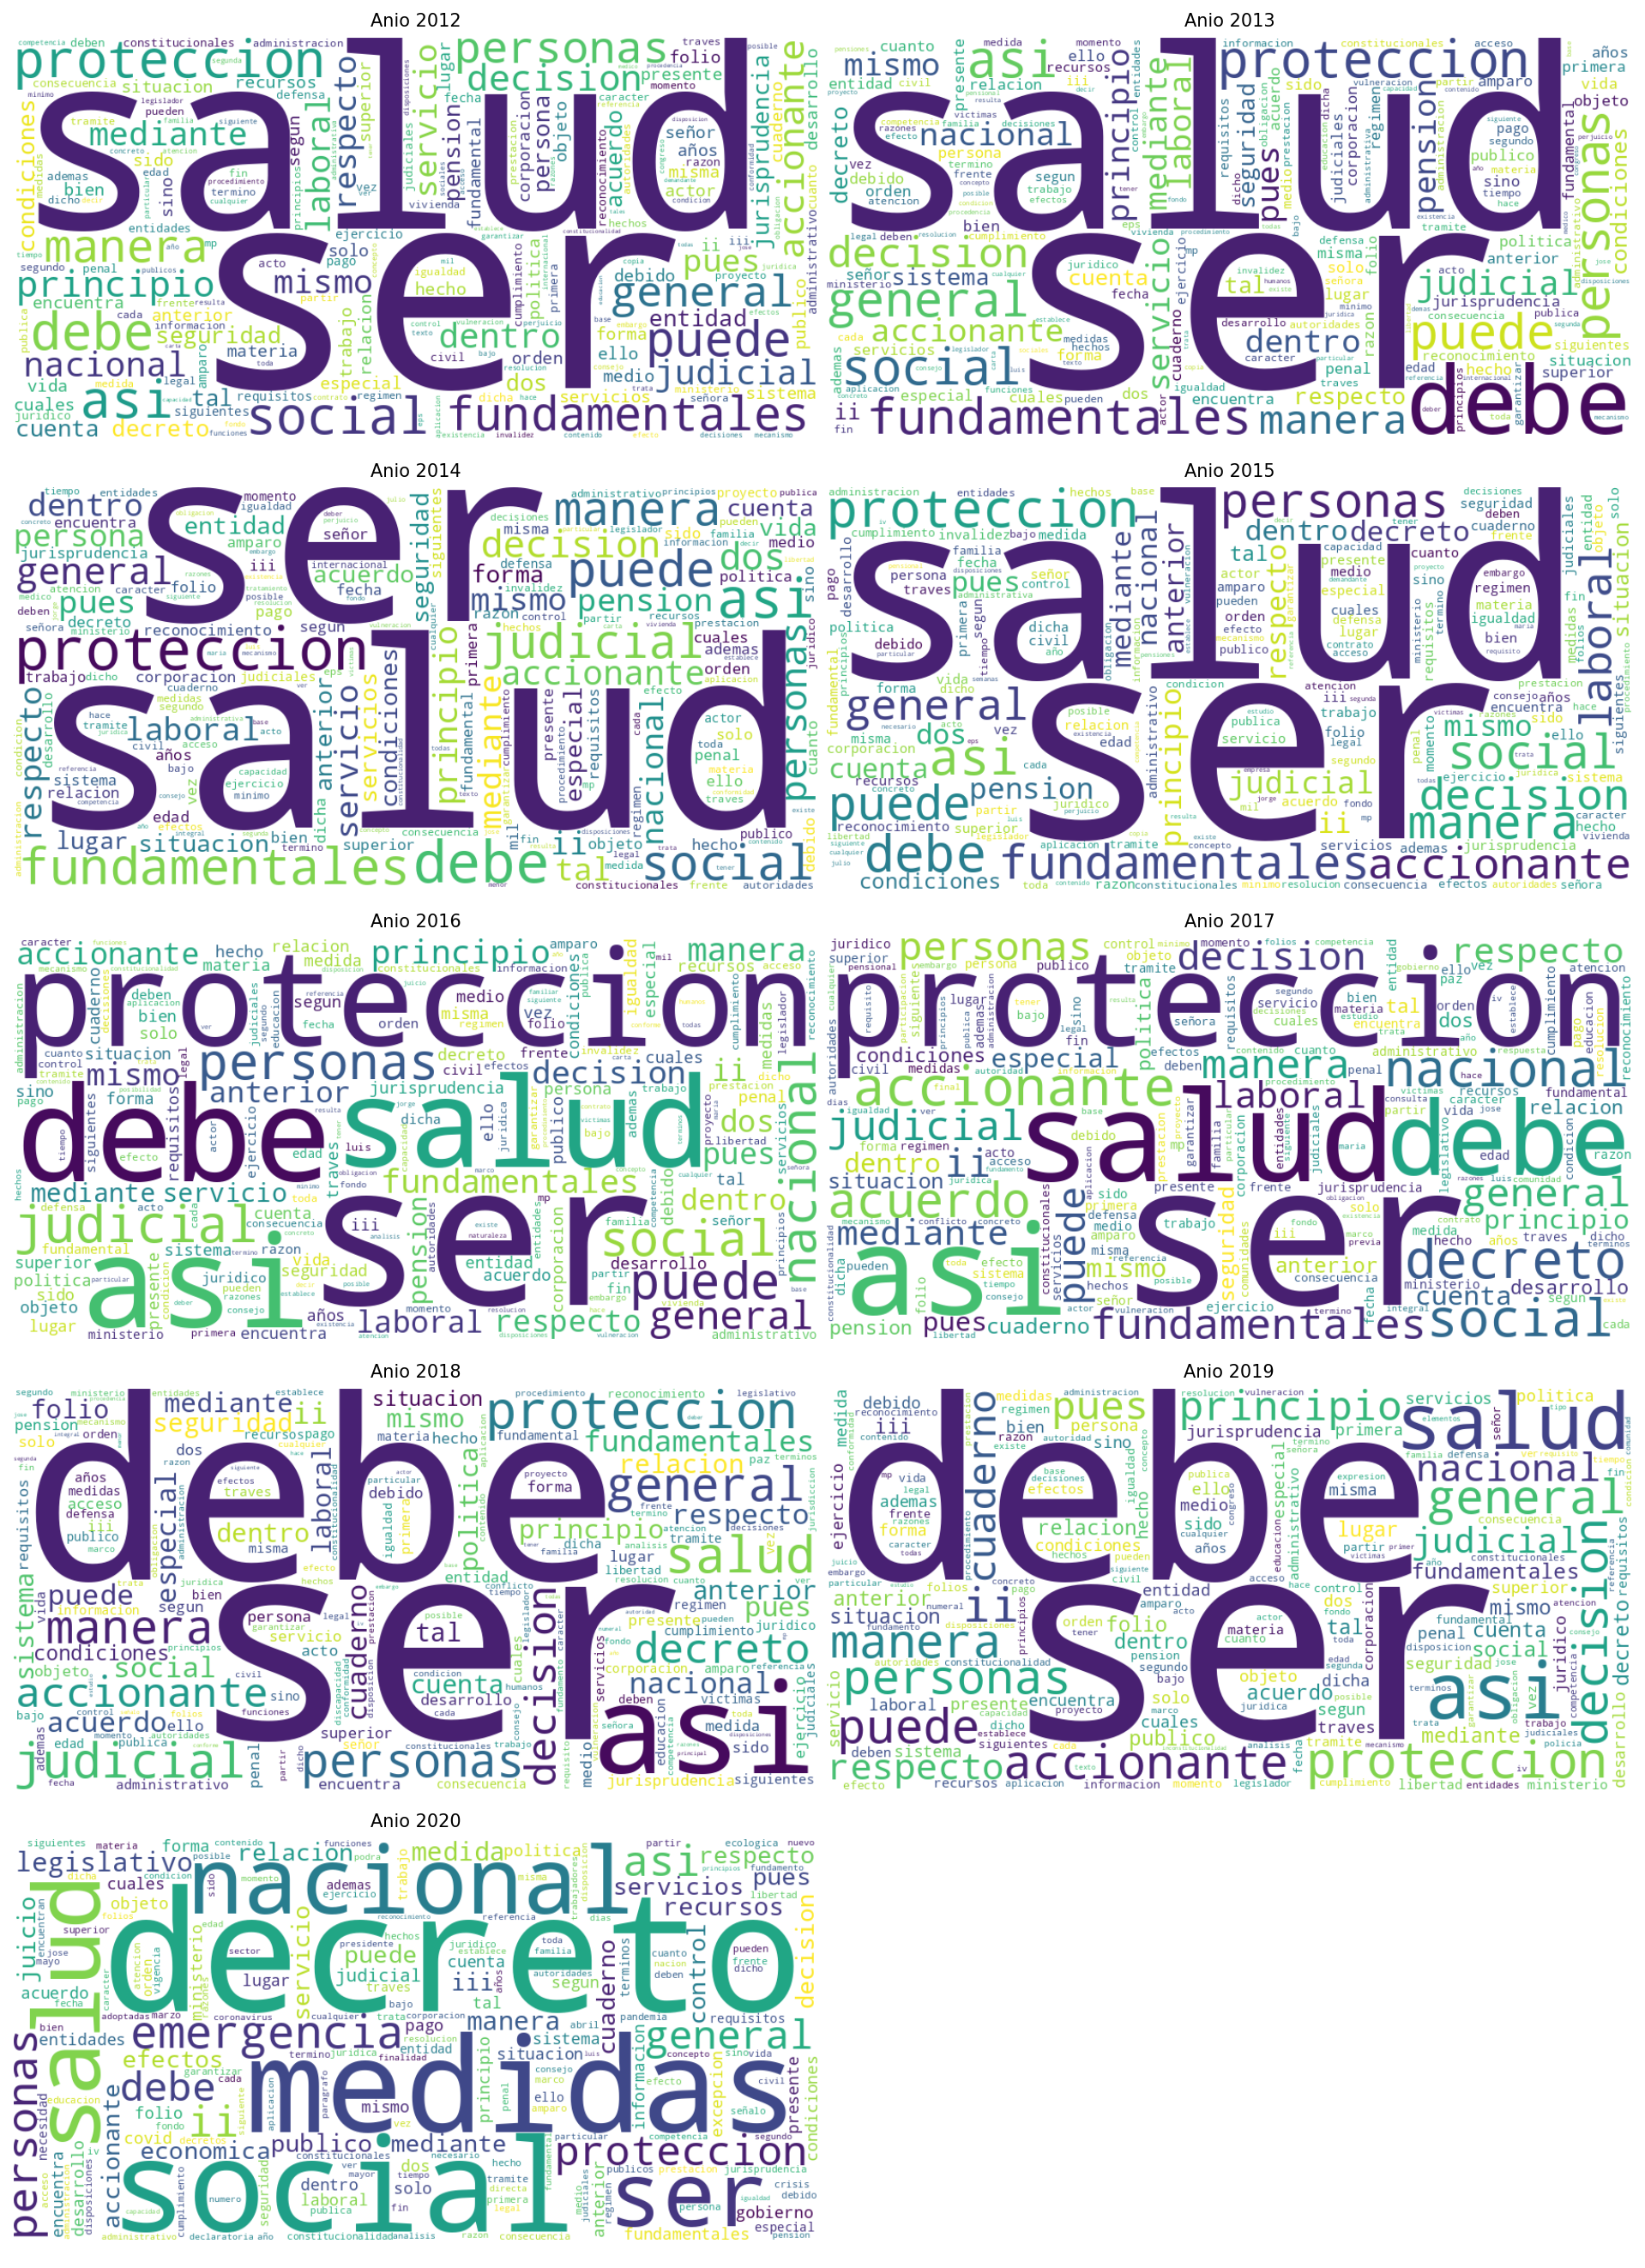
\includegraphics[width=\linewidth]{fig_nubes_por_anio_2012_2020.png}
        \caption{2012--2020.}
        \label{fig:nubes_p3}
    \end{subfigure}
    \caption{Nubes de palabras por año (sin palabras vacías gramaticales ni de dominio jurídico), en tres paneles.}
    \label{fig:nubes_periodos}
\end{figure}

\subsection{Recursos léxicos y ontologías}
\label{sec:ontologias}
El enunciado pide integrar, según el caso, ontologías, tesauros u otros recursos léxicos. Se evaluaron cuatro candidatas internacionales. (i) \textbf{EuroVoc / MultiEURLEX}: tesauro multilingüe con versión en español, utilizado en el corpus de 65.000 leyes de la Unión Europea etiquetadas con descriptores EUROVOC; es multietiqueta y documenta deriva conceptual temporal \cite{chalkidis2021multieurlex}. Su aplicabilidad es parcial: cubre derecho de la Unión Europea (reglamentos, directivas) y sus descriptores no mapean los títulos de la Constitución Política de 1991 ni el amparo de tutela. (ii) \textbf{LKIF} (\emph{Legal Knowledge Interchange Format}, OWL): ontología formal de conceptos jurídicos generales (norma, rol, acción, tiempo) del proyecto ESTRELLA, en inglés con partes en neerlandés; su aplicabilidad al español jurídico colombiano es baja, aunque sirve como patrón de modelado (separar norma, caso y rol). (iii) \textbf{ELI / ECLI}: esquemas europeos de identificación y metadatos de legislación y jurisprudencia; no son vocabularios temáticos y su aplicabilidad como ontología de contenido es nula, si bien inspiran identificadores estables de sentencias. (iv) \textbf{LegalRuleML / LegalDocML (Akoma Ntoso)}: lenguajes de marcado de reglas y de estructura documental; aportarían interoperabilidad, pero exigen anotación manual costosa y su aplicabilidad a corto plazo es baja.

La decisión documentada es no adoptar ninguna ontología externa tal cual para el dominio colombiano. En su lugar, se deriva una taxonomía ligera de la propia Constitución Política: los títulos y capítulos funcionan como bloques temáticos y los artículos 1--380 como etiquetas finas, con un mecanismo de respaldo (``derecho a X'') para las tutelas cuando la cita constitucional no está explícita. EuroVoc en español se conserva únicamente como referencia de comparación para la fase de clasificación, y LKIF se cita como patrón de modelado futuro. Esta decisión condiciona el diseño de etiquetas de la propuesta metodológica (sección \ref{sec:metodologia}) y se apoya, además, en la evidencia de que los corpus legales multilingües con etiquetas temáticas requieren protocolos de validación y particiones cronológicas por la deriva conceptual del dominio \cite{chalkidis2021multieurlex}.

\subsection{Granularidad del análisis}
\label{sec:granularidad}
Antes de fijar la unidad de análisis se evaluaron tres granularidades sobre una muestra estratificada de 600 documentos (20 por año disponible, semilla 42): sentencia completa, párrafo y subsentencia. Se definieron marcadores temáticos sobre el texto crudo: citas a la CP (patrón \emph{artículo N \ldots Constitución}, variantes con y sin tildes) más un respaldo de ``derecho a X''. El criterio se pre-registró antes de observar los resultados: la subsentencia solo se propondría como unidad si superaba en al menos 15 puntos porcentuales el porcentaje de unidades con marcador de la sentencia completa.

La tabla \ref{tab:granularidad} y la figura \ref{fig:granularidad} presentan el resultado. La sentencia completa contiene al menos un marcador en el 97,17\,\% de los casos (media de 20,03 marcadores por documento); la segmentación por párrafos no fragmentó los documentos ---el corpus no trae dobles saltos de línea: usa saltos simples, de modo que cada documento produce un único fragmento--- y por ello sus métricas coinciden con las de la sentencia; la fila ``párrafo'' es, por tanto, degenerada (párrafo $=$ sentencia), un hallazgo sobre el formato del corpus y no un error de cómputo. La subsentencia, en cambio, apenas alcanza un 4,64\,\% de unidades con marcador sobre 219.649 fragmentos. La comparación relevante (sentencia 97,17\,\% frente a subsentencia 4,64\,\%) no supera el criterio pre-registrado, de modo que se mantiene la sentencia completa como unidad de análisis. El experimento además deja ejemplos documentados de subsentencias con marcador (\texttt{ejemplos\_granularidad.md}), que muestran el tipo de fragmento que una segmentación recuperaría.

\begin{table}[htbp]
    \centering
    \caption{Granularidad del análisis: unidades, porcentaje con al menos un marcador temático y media de marcadores por unidad (muestra de 600 documentos).}
    \label{tab:granularidad}
    \begin{tabular}{lrrr}
        \toprule
        \textbf{Granularidad} & \textbf{Unidades} & \textbf{\% con marcador} & \textbf{Media de marcadores} \\
        \midrule
        Sentencia & 600 & 97,17\,\% & 20,03 \\
        Párrafo & 600 & 97,17\,\% & 20,03 \\
        Subsentencia & 219.649 & 4,64\,\% & 0,05 \\
        \bottomrule
    \end{tabular}
\end{table}

\begin{figure}[htbp]
    \centering
    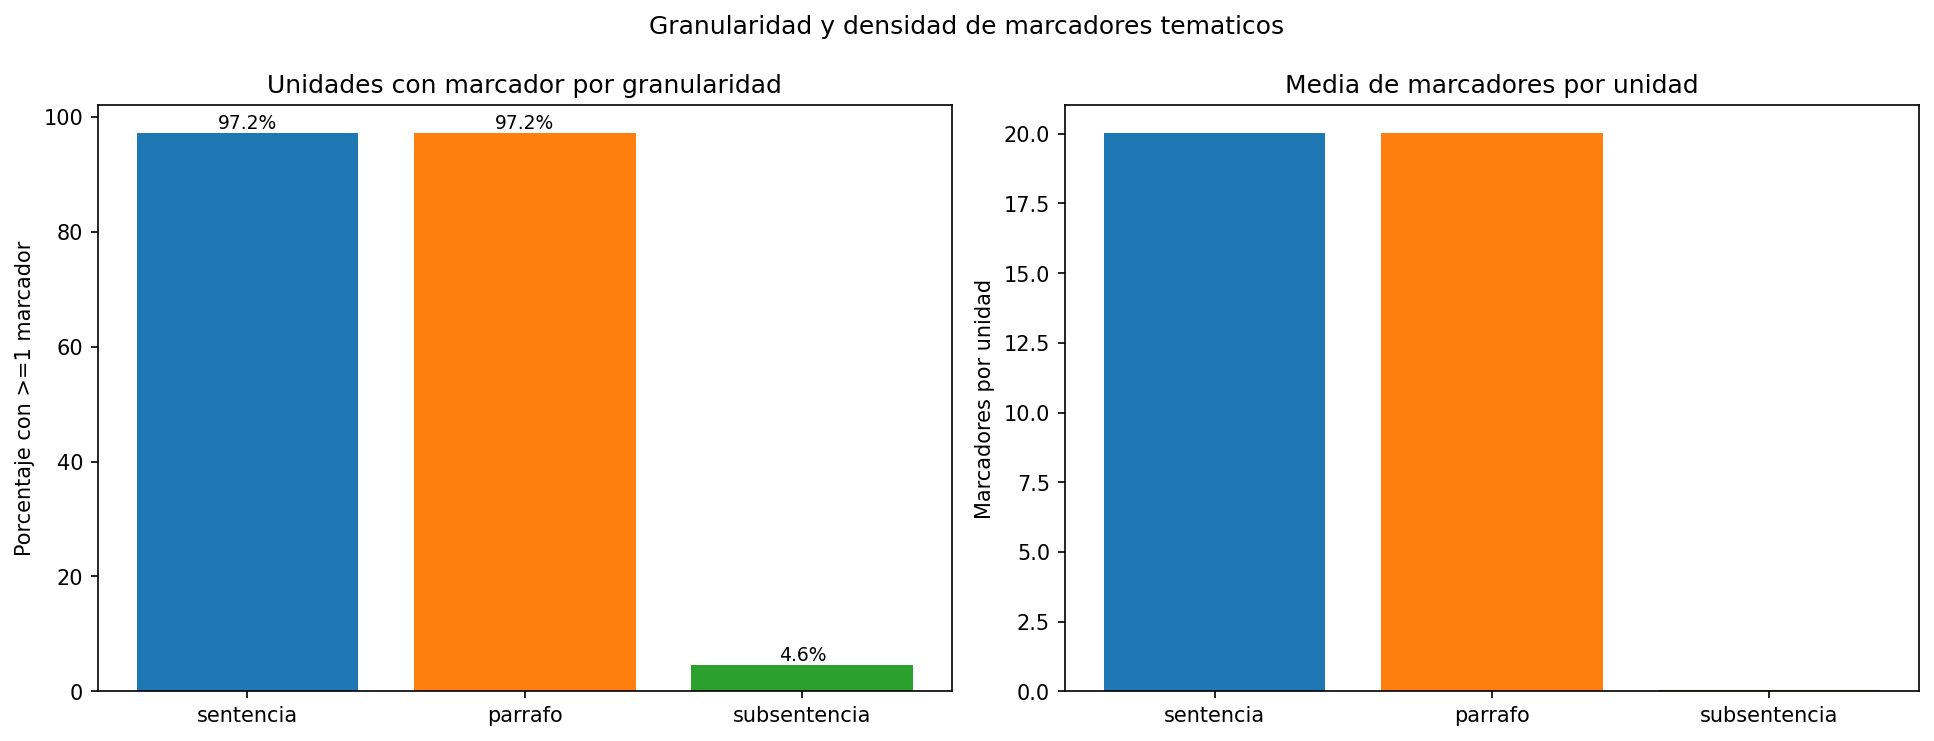
\includegraphics[width=0.78\linewidth]{fig_granularidad.png}
    \caption{Granularidad y densidad de marcadores temáticos: porcentaje de unidades con marcador (izquierda) y media de marcadores por unidad (derecha).}
    \label{fig:granularidad}
\end{figure}

Esta validación dialoga con la literatura que muestra que distintas secciones de una sentencia tienen distinto poder informativo para el modelado \cite{aletras2016predicting}: en este corpus, la señal temática disponible está distribuida a lo largo del documento completo y no concentrada en fragmentos cortos, lo que respalda tanto la unidad elegida como el uso de representaciones agregadas por documento (sección \ref{sec:representacion}).

% =====================================================================
% SECCION 5: REPRESENTACION DE LOS TEXTOS
% =====================================================================
\section{Representación de los textos}
\label{sec:representacion}

\subsection{Familias de representación y criterios de selección}
Las familias de representación consideradas fueron cuatro: (i) bolsa de palabras (BoW), que cuenta ocurrencias de términos; (ii) TF-IDF, que pondera los términos por su frecuencia y su especificidad documental; (iii) \emph{embeddings} estáticos (por ejemplo, vectores de palabra entrenados en un corpus), agregados a nivel de documento; y (iv) representaciones contextuales (\emph{transformers}), que codifican cada ocurrencia con su contexto. La elección se guio por cuatro criterios derivados del contexto del proyecto.

\textbf{Longitud de los documentos.} Las sentencias promedian $\approx$ 11.000 palabras y la mediana de lemas es de 7.116 (la mediana de palabras limpias es 7.158), muy por encima de la ventana de 512 \emph{tokens} de los \emph{transformers} estándar. Cualquier representación contextual exige segmentación con agregación de representaciones o truncamiento controlado, con la consiguiente pérdida de información; las representaciones de bolsa y TF-IDF no tienen ese límite.

\textbf{Interpretabilidad.} El proyecto busca ser una herramienta de apoyo a la consulta jurídica; los pesos de términos de TF-IDF permiten inspeccionar qué vocabulario sustenta cada categoría, mientras que las representaciones densas son opacas por construcción.

\textbf{Costo computacional.} TF-IDF sobre lemas se construye en minutos en CPU sobre los 23.742 documentos; el ajuste fino de un \emph{transformer} requiere GPU y presupuestos de cómputo mayores.

\textbf{Respaldo en la literatura.} La bolsa de palabras y TF-IDF siguen siendo líneas base fuertes en la clasificación de sentencias largas, donde los modelos neuronales no las superan de forma automática \cite{soh2019legalarea}; el preprocesamiento (normalización, palabras vacías, lematización) afecta de forma dependiente del corpus el rendimiento de las representaciones de bolsa \cite{hacohenKerner2020influence}; y los vocabularios jurídicos difieren del vocabulario general, lo que motiva tanto la adaptación de dominio como la evaluación de representaciones específicas \cite{chalkidis2020legalbert}. En corpus legales multilingües con etiquetas temáticas, las representaciones de términos se usan además como referencia para comparar transferencia entre lenguas y deriva temporal \cite{chalkidis2021multieurlex}.

\subsection{Bolsa de palabras y TF-IDF}
La representación de bolsa de palabras describe cada documento $d$ como un vector $\mathbf{x}_d \in \mathbb{N}^{|V|}$ sobre un vocabulario $V$, donde la componente del término $t$ es el número de ocurrencias de $t$ en $d$. Su limitación principal es que ignora el orden y la composición de las palabras, pero en un género con fórmulas estables como el judicial conserva una señal léxica potente. La ponderación TF-IDF atenúa el peso de los términos muy frecuentes en el corpus y realza los específicos de cada documento \cite{manning2008introduction}. Concretamente, se emplea la variante de frecuencia sublineal
\begin{equation}
\mathrm{tf}(t,d) =
\begin{cases}
1 + \log \mathrm{c}(t,d), & \mathrm{c}(t,d) > 0,\\
0, & \mathrm{c}(t,d) = 0,
\end{cases}
\label{eq:tf}
\end{equation}
donde $\mathrm{c}(t,d)$ es el conteo bruto del término; la frecuencia inversa de documento
\begin{equation}
\mathrm{idf}(t) = \log \frac{N}{\mathrm{df}(t)},
\label{eq:idf}
\end{equation}
con $N$ el número de documentos y $\mathrm{df}(t)$ el número de documentos que contienen $t$; y el peso final
\begin{equation}
w(t,d) = \mathrm{tf}(t,d)\cdot \mathrm{idf}(t),
\label{eq:tfidf}
\end{equation}
seguido de una normalización $\ell_2$ del vector, $\mathbf{x}_d \leftarrow \mathbf{x}_d / \lVert \mathbf{x}_d \rVert_2$, que evita que los documentos largos dominen las comparaciones por magnitud. La extensión a n-gramas consiste en tratar cada secuencia de 1--2 términos consecutivos como una dimensión adicional del vocabulario, lo que captura fórmulas del género (\emph{accion de tutela}, \emph{debido proceso}) que el unigrama no distingue.

\subsection{Ejemplos de vectorización}
\label{sec:vectorizacion}
La representación se ajustó sobre los 23.742 documentos lematizados con la configuración de la sección \ref{sec:decision} y produjo una matriz dispersa de 23.742 $\times$ 100.000 rasgos con 103.045.759 valores no nulos, es decir, una esparsidad del 95,66\,\%; el ajuste tardó $\approx$ 212 segundos en CPU (211,9 s en el notebook ejecutado). Por documento, el vector activa en promedio 4.340 rasgos (mediana 3.717,5; mínimo 378; máximo 37.320) y su norma $\ell_2$ es 1 por la normalización, lo que hace comparables documentos de longitudes muy distintas. La figura \ref{fig:tfidf} muestra dos vistas de la representación: la cola larga del vocabulario ---$\approx$2\,\% de la masa de frecuencia documental se concentra en los 100 primeros rasgos, $\approx$17\,\% en los 1.000 y $\approx$60\,\% en los 10.000--- y los 15 rasgos de mayor peso del documento T representativo.

Para hacer tangible la transformación texto $\rightarrow$ vector se eligieron tres documentos con un criterio estable e independiente de resultados de modelos: el identificador mínimo de cada tipo. La tabla \ref{tab:vectorizacion} resume sus 15 rasgos de mayor peso y sus dimensiones efectivas: T-001/2021 (id 0) activa 7.712 rasgos, C-022/2021 (id 14) 11.027 y SU-016/2021 (id 19) 15.820. Los términos principales son específicos de cada caso (\emph{capital salud}, \emph{salud mental}, \emph{pañal} en la tutela; \emph{cdpd}, \emph{capacidad legal}, \emph{persona titular} en la de constitucionalidad; \emph{el copey}, \emph{desalojo}, \emph{uariv} en la de unificación), coherentes con el contenido jurídico de cada providencia. La similitud coseno entre los tres vectores es baja (0,242 entre T y C; 0,253 entre T y SU; 0,251 entre C y SU): documentos de materias distintas comparten solo el vocabulario genérico del género. El contraste entre conteo bruto y TF-IDF para el documento T ilustra la ponderación sublineal: \emph{capital salud} aparece 35 veces y recibe peso 0,065, mientras \emph{salud mental} aparece 75 veces y recibe 0,049, porque su frecuencia inversa de documento es menor.

\begin{table}[htbp]
    \centering
    \caption{Top-15 rasgos de mayor peso TF-IDF para los tres documentos representativos (peso entre paréntesis, redondeado a tres decimales). Algunos rasgos son siglas o abreviaturas del corpus (p.~ej., \emph{cdpd}, \emph{eci}), conservadas tal como aparecen en los datos.}
    \label{tab:vectorizacion}
    \small
    \begin{tabular}{cp{0.28\textwidth}p{0.28\textwidth}p{0.28\textwidth}}
        \toprule
        \textbf{\#} & \textbf{T-001/2021 (id 0)} & \textbf{C-022/2021 (id 14)} & \textbf{SU-016/2021 (id 19)} \\
        \midrule
        1 & capital salud (0,065) & cdpd (0,050) & el copey (0,054) \\
        2 & valero (0,056) & pg (0,048) & copey (0,053) \\
        3 & de calle (0,052) & persona titular (0,048) & eci (0,041) \\
        4 & salud mental (0,049) & capacidad legal (0,047) & de desalojo (0,038) \\
        5 & folio historia (0,046) & el cdpd (0,046) & desalojo (0,036) \\
        6 & sustancia psicoactiva (0,046) & top (0,040) & albergue temporal (0,035) \\
        7 & jhon (0,046) & capacidad jurídico (0,040) & no reportar (0,034) \\
        8 & psicoactiva (0,046) & sv (0,038) & el uariv (0,034) \\
        9 & trastorno mental (0,046) & correa spv (0,038) & el ocupante (0,034) \\
        10 & úlcera (0,045) & como apoyo (0,037) & uariv (0,033) \\
        11 & pañal (0,045) & con discapacidad (0,037) & venezolano (0,033) \\
        12 & pañal desechabl (0,044) & preferencia de (0,036) & desalojo en (0,033) \\
        13 & habilitación rehabilitación (0,044) & inhabilitación (0,035) & ocupante (0,033) \\
        14 & desechabl (0,043) & personalidad jurídico (0,035) & vivienda gratuito (0,033) \\
        15 & el pañal (0,042) & ley estatutario (0,035) & albergue (0,033) \\
        \bottomrule
    \end{tabular}
\end{table}

\begin{figure}[htbp]
    \centering
    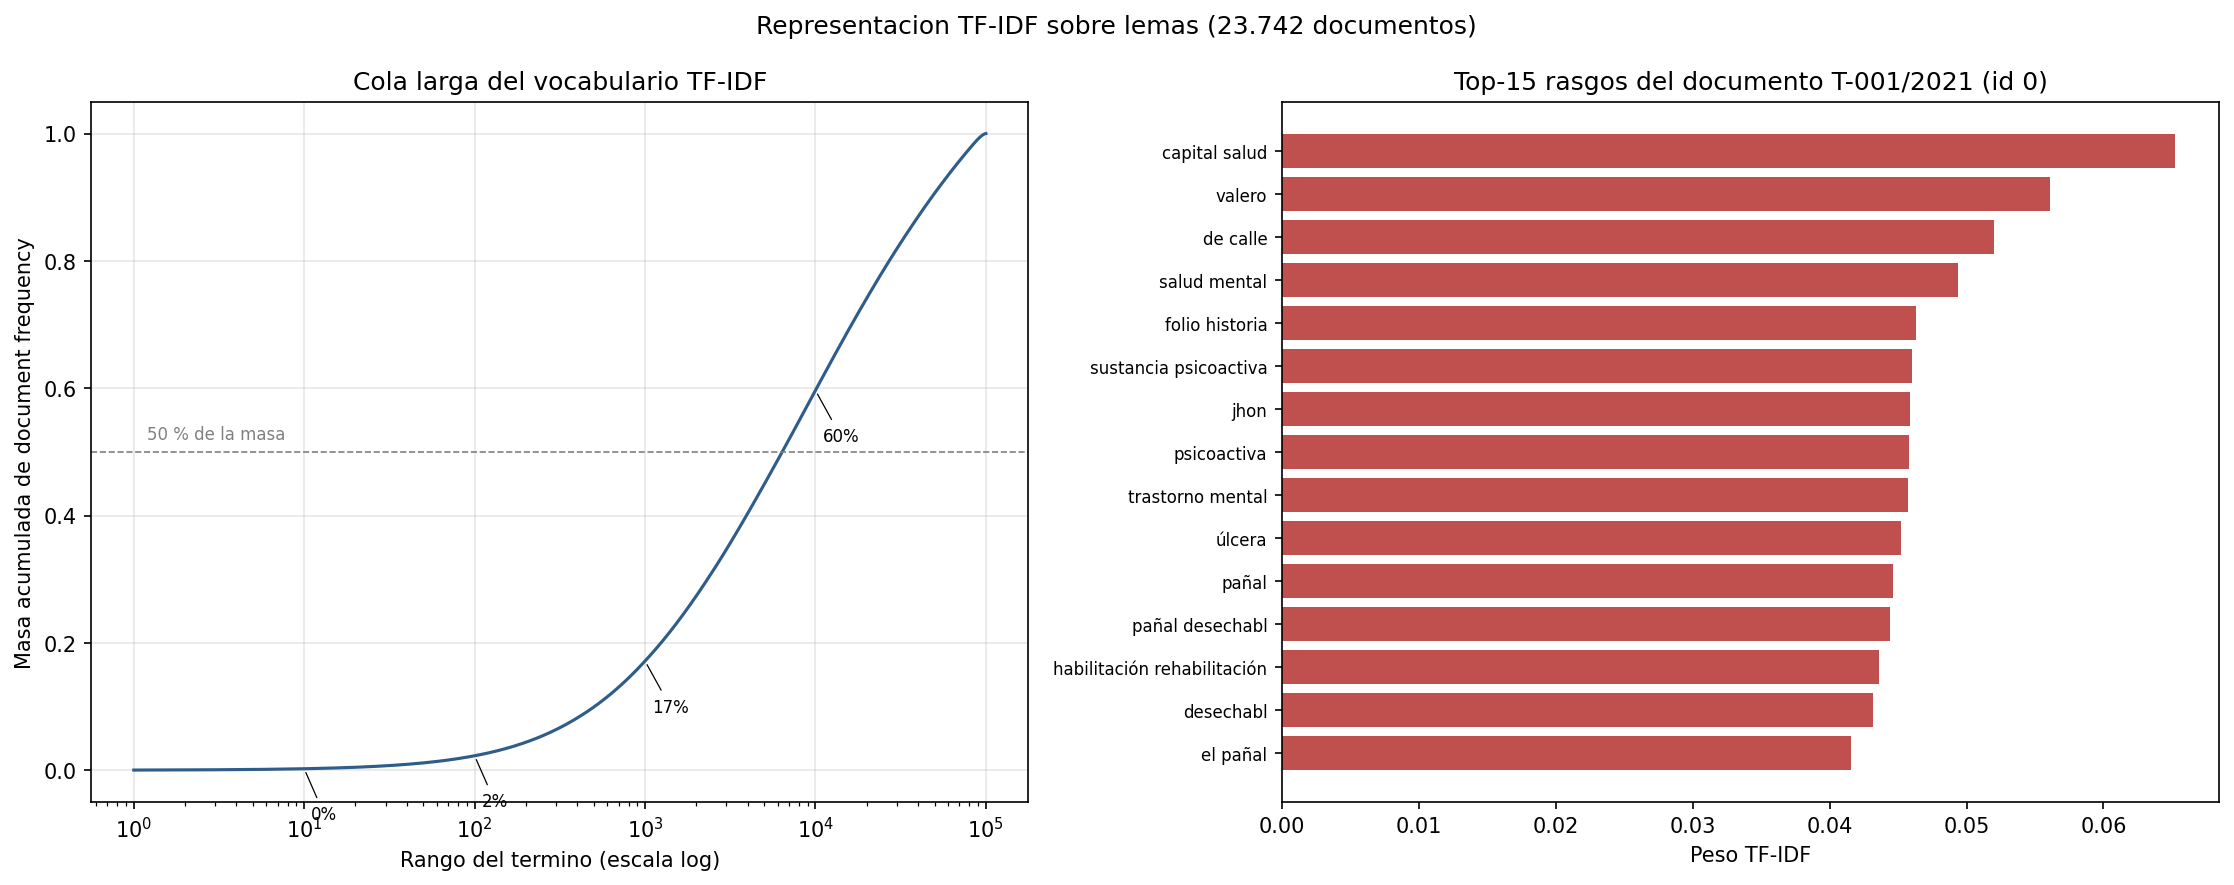
\includegraphics[width=0.70\linewidth]{fig_representacion_tfidf.png}
    \caption{Representación TF-IDF sobre lemas (23.742 documentos): cola larga del vocabulario (izquierda) y top-15 rasgos del documento T-001/2021 (derecha).}
    \label{fig:tfidf}
\end{figure}

\subsection{\emph{Embeddings} y representaciones contextuales}
Las representaciones densas se consideran complementarias para este proyecto. Los \emph{embeddings} estáticos asignan a cada palabra un vector entrenado y el documento se representa agregando (media o suma ponderada) los vectores de sus palabras; los modelos contextuales, en cambio, producen representaciones dependientes del contexto, y las variantes tipo \emph{Sentence-BERT} permiten obtener vectores de fragmento comparables por similitud coseno con un costo de inferencia muy inferior al de comparar pares con BERT completo \cite{reimers2019sentencebert}. Para el español existen adaptaciones del esquema BERT preentrenadas en este idioma (p.~ej., BETO) y variantes de dominio legal como LEGAL-BERT, que muestran que el vocabulario jurídico difiere del general \cite{chalkidis2020legalbert}. Su utilidad esperada en el proyecto es doble: comparación semántica entre sentencias y apoyo a la recuperación de fragmentos relevantes. Su adopción como representación principal choca, sin embargo, con la longitud de los documentos ($\approx$ 11.000 palabras frente a ventanas de 512 \emph{tokens}), la opacidad de los vectores y el costo de cómputo; por eso se reservan para experimentos comparativos de la fase de modelado.

La demostración con \emph{embeddings} contextuales se ejecutó con \emph{intfloat/multilingual-e5-base} (768 dimensiones) sobre cinco documentos codificados con sus primeros 512 \emph{tokens} y el prefijo \texttt{query:} en ambos lados de la comparación (similitud simétrica), en GPU. La figura \ref{fig:embeddings} presenta la matriz de similitud coseno resultante: los documentos de 2021 mantienen similitudes altas entre sí (0,907--0,926) y el documento de 1992 se separa ligeramente (0,870--0,878); la similitud media es 0,899. La comparación con la representación dispersa es instructiva: para los mismos tres documentos representativos, la similitud coseno es de 0,91--0,92 con los \emph{embeddings} y de 0,24--0,25 con TF-IDF. Los \emph{embeddings} contextuales capturan una cercanía semántica y estilística general ---con valores típicamente altos y comprimidos, que exigen cautela al fijar umbrales---, mientras que TF-IDF discrimina por solapamiento léxico y es auditable término a término. Ambas vistas son complementarias y así se usarán en la fase de modelado.

\begin{figure}[htbp]
    \centering
    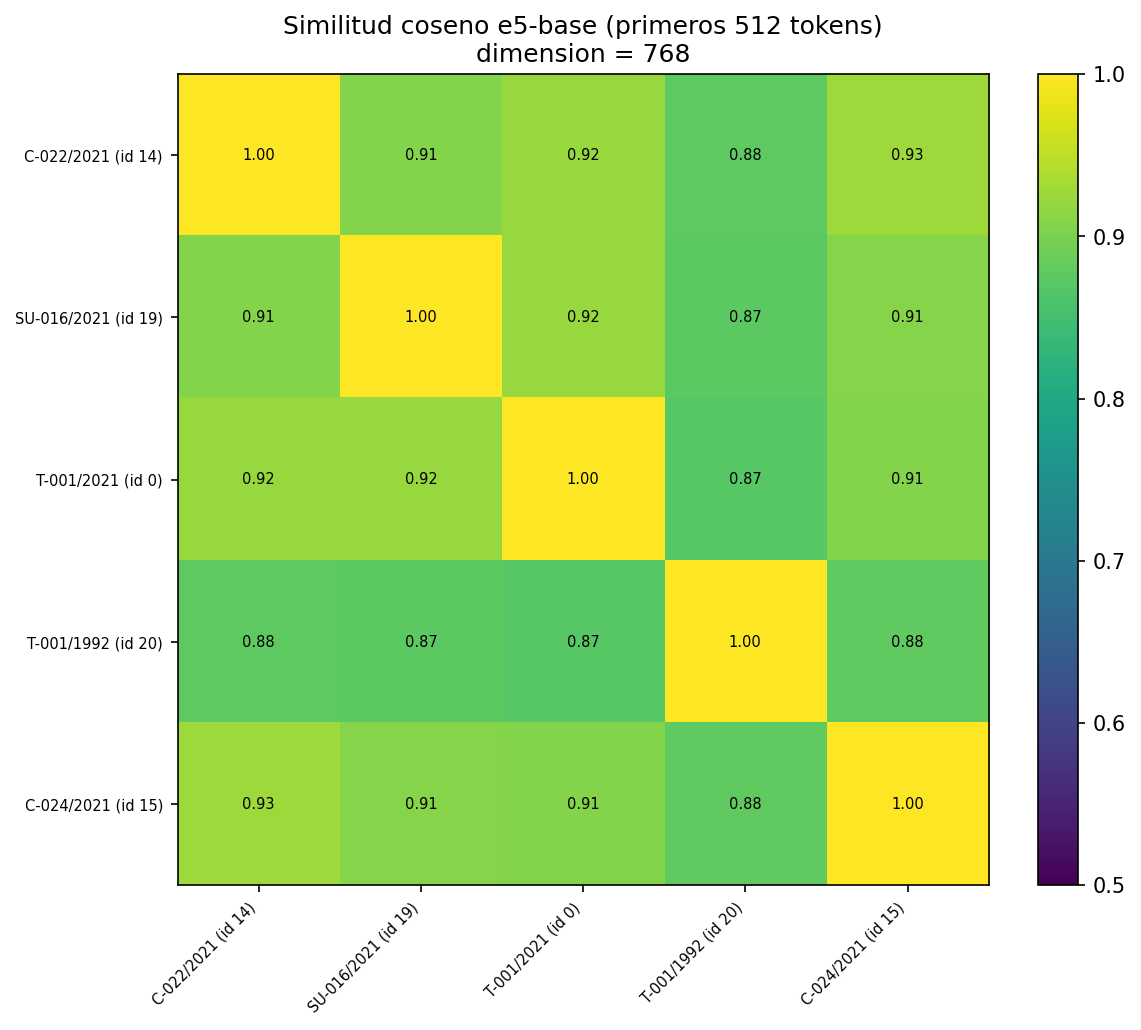
\includegraphics[width=0.52\linewidth]{fig_embeddings_ejemplo.png}
    \caption{Similitud coseno entre cinco documentos codificados con \emph{multilingual-e5-base} (primeros 512 \emph{tokens}; dimensión 768).}
    \label{fig:embeddings}
\end{figure}

\subsection{Decisión: TF-IDF sobre lemas}
\label{sec:decision}
La representación principal del proyecto será \textbf{TF-IDF sobre lemas} con las siguientes características: rasgos de 1--2 lemas (\texttt{ngram\_range=(1,2)}), frecuencia mínima documental de 3 (\texttt{min\_df=3}), vocabulario máximo de 100.000 rasgos (\texttt{max\_features=100000}) y frecuencia sublineal (\texttt{sublinear\_tf=True}), sobre los 23.742 documentos del corpus medido (el ajuste efectivo tardó $\approx$ 212 segundos y produjo una esparsidad del 95,66\,\%; sección \ref{sec:vectorizacion}). La decisión se justifica en cuatro puntos. Primero, los pesos de términos son interpretables: cada categoría puede auditarse inspeccionando los lemas de mayor peso, requisito deseable en una herramienta jurídica. Segundo, la lematización reduce el vocabulario en un 12,7\,\% y agrupa flexiones (\emph{derechos}/\emph{derecho}) sin sacrificar legibilidad, a diferencia del \emph{stemming} (sección \ref{sec:morfologia}). Tercero, la literatura reporta que las representaciones de bolsa con ponderación TF-IDF son líneas base competitivas en la clasificación de sentencias largas \cite{soh2019legalarea} y que su rendimiento depende críticamente del preprocesamiento documentado \cite{hacohenKerner2020influence}. Cuarto, su costo es mínimo frente a las alternativas contextuales, lo que permite reservar el presupuesto de cómputo para la comparación experimental de la fase final (sección \ref{sec:metodologia}). El vectorizador se ajustará exclusivamente con el conjunto de entrenamiento, de modo que el vocabulario y las ponderaciones IDF no incorporen información del conjunto de prueba (sección \ref{sec:particiones}).

% =====================================================================
% SECCION 6: PROPUESTA METODOLOGICA
% =====================================================================
\section{Propuesta metodológica}
\label{sec:metodologia}

\subsection{Tarea y enfoque}
La tarea propuesta es una \textbf{clasificación supervisada multi-clase} de sentencias. Se distinguen dos niveles de etiquetas. El primero, inmediato, es el \emph{tipo de providencia} (T, C o SU), que se extrae del encabezado del documento y funciona como categoría inicial: es una tarea de tres clases, útil como banco de pruebas del \emph{pipeline} completo (representación, particiones, métricas) y como línea base interpretable. El segundo, objetivo principal del proyecto, es el \emph{área temática constitucional} de la sentencia, derivada de la taxonomía ligera construida a partir de la Constitución Política (títulos y capítulos como bloques temáticos, artículos como etiquetas finas y respaldo ``derecho a X'' para tutelas; sección \ref{sec:ontologias}). Estas etiquetas temáticas están por validar: la propuesta contempla que su definición final y su anotación se sometan a un protocolo de validación antes de usarlas como variable dependiente, y que se documente su procedencia.

La clasificación supervisada es adecuada porque el objetivo del sistema es asignar categorías a documentos completos, tarea para la que existen antecedentes directos en sentencias judiciales: la comparación de clasificadores clásicos y neuronales sobre sentencias largas de la Corte Suprema de Singapur \cite{soh2019legalarea}, los \emph{pipelines} de clasificación de sentencias en español con categorías dependientes de la jurisdicción \cite{gonzalezGonzalez2023automatic} y la clasificación multietiqueta de documentos legales multilingües con etiquetas de tesauro \cite{chalkidis2021multieurlex}. La naturaleza del área temática (una sentencia puede invocar varios bloques constitucionales) sugiere evaluar, en una segunda iteración, la formulación multi-etiqueta; la primera iteración se plantea multi-clase para obtener una línea base simple y auditable.

\subsection{Datos, particiones y criterios anti-\emph{leakage}}
\label{sec:particiones}
El insumo es el conjunto de datos medido (sección \ref{sec:dataset}) y su representación TF-IDF sobre lemas (sección \ref{sec:decision}). La partición propuesta es \textbf{70/15/15 estratificada} por clase, con semilla fija 42: 70\,\% entrenamiento, 15\,\% validación y 15\,\% prueba. La estratificación se aplica por tipo de providencia y se verifica por año, para evitar que los periodos con menos documentos queden sobrerrepresentados en algún subconjunto. El conjunto de prueba permanece \emph{intocable} durante el desarrollo: todas las decisiones de representación, hiperparámetros y selección de modelo se toman con entrenamiento y validación, y el conjunto de prueba se usa una única vez al final para reportar el desempeño.

Los criterios anti-\emph{leakage} son parte constitutiva del diseño: (i) la partición es a nivel de documento, nunca de fragmentos, de modo que ninguna parte de una sentencia aparece simultáneamente en entrenamiento y prueba; (ii) el vocabulario y las ponderaciones IDF del vectorizador se ajustan solo con el conjunto de entrenamiento y luego se aplican a validación y prueba; (iii) los pasos de preprocesamiento (normalización, palabras vacías, lematización) son transformaciones fijas y no aprendidas del corpus de prueba; (iv) la selección de hiperparámetros y de modelo se realiza exclusivamente con la métrica de validación; y (v) dada la naturaleza formulaica del corpus, se verificarán duplicados y casi duplicados antes de fijar las particiones. Adicionalmente, por la deriva léxica documentada entre periodos (secciones \ref{sec:mtld} y \ref{sec:periodos}) y por la evidencia de que los corpus legales exigen particiones cronológicas para medir generalización temporal \cite{chalkidis2021multieurlex}, se contempla una partición cronológica complementaria (entrenar con los periodos antiguos y evaluar en los recientes) como análisis de robustez, sin reemplazar la partición aleatoria estratificada principal.

\subsection{Modelos a comparar y criterios de evaluación}
Se comparan tres niveles de modelos, de menor a mayor costo. (1) \textbf{Línea base mayoritaria}: asignar siempre la clase más frecuente; fija el piso de comparación y permite cuantificar cuánto aporta la representación. (2) \textbf{Línea base clásica}: TF-IDF sobre lemas con modelos lineales (regresión logística multinomial y máquina de vectores de soporte lineal), entrenados sobre los rasgos definidos en la sección \ref{sec:decision}. (3) \textbf{\emph{Transformer} contextual en español}: ajuste fino de un modelo tipo BETO con segmentación del documento en fragmentos de 512 \emph{tokens} y agregación de las representaciones (media de fragmentos) para obtener una representación por documento; el modelo de dominio legal se considera como variante si el presupuesto lo permite \cite{chalkidis2020legalbert}.

Los criterios de evaluación son: \emph{macro-F1} como métrica principal (dado el desbalance entre clases, con T en el 72,02\,\% de los documentos), F1 por clase con precisión y \emph{recall}, matriz de confusión, análisis cualitativo de errores (revisión de las confusiones más frecuentes sobre los documentos mal clasificados) y evaluación por cortes (desempeño por tipo de providencia y por periodo, para detectar degradación temporal). En cuanto al costo, se registran tiempos de entrenamiento e inferencia, memoria y requerimiento de GPU, con el fin de que la comparación no premie únicamente la métrica sino la viabilidad operativa. La tabla \ref{tab:modelos} resume la comparación propuesta.

\begin{table}[htbp]
    \centering
    \caption{Modelos a comparar y criterios de evaluación de la fase de modelado.}
    \label{tab:modelos}
    \small
    \begin{tabular}{p{0.17\textwidth}p{0.19\textwidth}p{0.23\textwidth}p{0.27\textwidth}}
        \toprule
        \textbf{Enfoque} & \textbf{Representación} & \textbf{Fortalezas} & \textbf{Límites esperados y criterios} \\
        \midrule
        Línea base mayoritaria & --- & piso de comparación; costo nulo & no aporta información; macro-F1 y F1 por clase \\
        Clásica: modelos lineales & TF-IDF sobre lemas (1--2 gramos) & interpretable; bajo costo; robusta en documentos largos & pierde orden y composicionalidad; macro-F1, matriz de confusión, análisis de errores, costo \\
        \emph{Transformer} en español & BETO con segmentación y agregación & contexto y composicionalidad; estado del arte & costo de GPU; ventana de 512; requiere segmentación; macro-F1, F1 por clase, robustez por periodo, costo \\
        \bottomrule
    \end{tabular}
\end{table}

\subsection{Riesgos y mitigaciones}
\textbf{Desbalance de clases.} Las tutelas dominan el corpus (72,02\,\%). Mitigación: particiones estratificadas, macro-F1 como métrica principal y ponderación de clases en el entrenamiento (solo con el conjunto de entrenamiento), además de reportar el desempeño por clase para evitar que la clase mayoritaria oculte fallos en C y SU.

\textbf{Documentos largos frente a la ventana del \emph{transformer}.} Con $\approx$ 11.000 palabras por sentencia, el truncamiento simple descarta la mayor parte del contenido. Mitigación: segmentación en fragmentos con agregación de representaciones y comparación explícita con la línea base TF-IDF, que no sufre este límite.

\textbf{Etiquetas temáticas por validar.} La taxonomía derivada de la CP es una construcción del proyecto y no un recurso anotado por terceros. Mitigación: protocolo de validación con anotación (al menos una muestra revisada por personas expertas), documentación de la procedencia de cada etiqueta y reporte del acuerdo entre anotadores; mientras la validación no esté cerrada, el tipo de providencia funciona como etiqueta de referencia para el desarrollo del \emph{pipeline}. La escasez de recursos legales anotados en español para América Latina \cite{loffler2025predicting} refuerza la importancia de documentar esta validación.

\textbf{Deriva temporal y composición por periodo.} El vocabulario y la diversidad léxica cambian entre 1992 y 2021 (secciones \ref{sec:mtld} y \ref{sec:periodos}). Mitigación: evaluación por cortes temporales y partición cronológica complementaria, y reporte del desempeño por periodo junto al desempeño global.

\textbf{Duplicados y plantillas.} El género es formulaico y pueden existir documentos casi idénticos. Mitigación: verificación de duplicados y casi duplicados antes de fijar las particiones y análisis de errores consciente de plantillas (por ejemplo, revisar si los errores se concentran en documentos atípicos).

\textbf{Costo computacional.} El ajuste fino de un \emph{transformer} consume GPU y tiempo. Mitigación: la línea base clásica corre en CPU y se ejecuta primero; el \emph{transformer} se reserva para una comparación acotada (un modelo, presupuesto de cómputo definido) y su inclusión no bloquea el resto de la metodología.

\subsection{Trabajo futuro}
El trabajo posterior a esta entrega comprende: (i) cerrar la validación de las etiquetas temáticas y documentar su calidad; (ii) ejecutar la comparación de modelos con el protocolo de particiones y métricas aquí definido; (iii) profundizar el análisis de errores por periodo y por tipo; (iv) evaluar representaciones densas y de dominio legal como complemento de TF-IDF para la comparación semántica y la recuperación de fragmentos; y (v) explorar componentes de apoyo a la consulta de sentencias extensas (resúmenes y extracción de información), en línea con los objetivos del proyecto.

% =====================================================================
% SECCION 7: CONCLUSIONES
% =====================================================================
\section{Conclusiones}
\label{sec:conclusiones}

Esta entrega profundizó el análisis del corpus de 23.742 sentencias de la Corte Constitucional de Colombia (1992--2021) y dejó definidas la representación de los textos y la metodología de modelado del proyecto. En primer lugar, se documentaron y verificaron las modificaciones respecto a la Entrega 1: el corpus se persiste ahora como conjunto de datos medido (\texttt{corpus\_medido.parquet}) con texto, texto limpio y métricas por documento; el EDA avanzado ---n-gramas y colocaciones, lemas/\emph{stems}, POS, MTLD, granularidad y recursos léxicos--- se incorporó con su lectura analítica; la unidad de análisis (sentencia completa) quedó validada con un experimento pre-registrado; y se cumplió la promesa del análisis por periodos, además de formularse por primera vez la representación y la propuesta metodológica. Las cifras canónicas del corpus no requirieron corrección.

En segundo lugar, el EDA avanzado caracterizó el género con evidencia cuantitativa: el corpus es fuertemente formulaico (\emph{accion de tutela} es el trigrama más frecuente, con 344.893 ocurrencias; el 82,7\,\% de los trigramas guardados responden al patrón con palabra intermedia vacía); la razón de verosimilitud es la medida de asociación más confiable para las colocaciones (75\,\% de fórmulas válidas frente a 55\,\% de la frecuencia y 0\,\% del PMI); la diversidad léxica desciende sostenidamente de 64,32 (1992--2001) a 58,53 (2012--2021), con una pendiente de $-0,32$ puntos por año; el contraste por periodos muestra un recambio temático del vocabulario, de las siglas institucionales del primer bloque (\emph{incoder}, \emph{rupd}) al léxico del conflicto armado y la pandemia en la última década (\emph{uariv}, \emph{jep}, \emph{coronavirus}); la lematización reduce el vocabulario en un 12,7\,\% conservando legibilidad; y la señal temática está distribuida en el documento completo (97,17\,\% de sentencias con marcador frente a 4,64\,\% de subsentencias). La evaluación de recursos léxicos concluyó que ninguna ontología externa cubre el dominio colombiano, por lo que se deriva una taxonomía ligera de la propia Constitución Política.

En tercer lugar, se seleccionó y calculó TF-IDF sobre lemas (rasgos de 1--2 lemas, frecuencia mínima documental de 3, hasta 100.000 rasgos y ponderación sublineal) como representación principal ---matriz de 23.742 $\times$ 100.000 rasgos con 95,66\,\% de esparsidad---, por su interpretabilidad, su bajo costo y su respaldo en la literatura de clasificación de sentencias largas, y se propuso una metodología de clasificación supervisada multi-clase con particiones 70/15/15 estratificadas (semilla 42, prueba intocable), criterios anti-\emph{leakage} explícitos y comparación entre modelos lineales y \emph{transformers} en español bajo criterios de macro-F1, F1 por clase, análisis de errores y costo. El conjunto de datos medido, el EDA avanzado y la propuesta metodológica dejan al proyecto en condiciones de iniciar su fase de modelado con insumos trazables y decisiones justificadas.

% =====================================================================
% BIBLIOGRAFIA (estilo apalike; todas las claves citadas existen en
% references.bib y todas las entradas del .bib se citan en el texto)
% =====================================================================
\bibliographystyle{apalike}
{\small\bibliography{references}}

\end{document}
